\documentclass[10pt,aspectratio=43]{beamer}		
\usefonttheme{professionalfonts}

\mode<presentation>

\usepackage{NUSTM}

% % math support
\usepackage{latexsym}
\usepackage{siunitx}
\usepackage{newtxtext}
\usepackage{newtxmath}
\usepackage{amsmath}
\usepackage{amsfonts}
\usepackage{amssymb}
\usepackage{amsthm}
\newcommand\bmmax{2}
\usepackage{bm}
\usepackage{physics}

% table support
\usepackage{arydshln} % for dashed line in tables
\usepackage{multirow}
\usepackage{makecell}

% commonly used packages
\usepackage{color}
\usepackage{xcolor}
\usepackage{graphicx}
\usepackage{hyperref}
\usepackage{url}
\usepackage{times}
\usepackage{verbatim}
\usepackage{xspace}
\usepackage{microtype}

% bibliography support
\usepackage[square, numbers]{natbib}
\setbeamertemplate{bibliography item}[text]

% highlighting support
\usepackage{soul}
\makeatletter
\let\HL\hl
\renewcommand\hl{%
  \let\set@color\beamerorig@set@color
  \let\reset@color\beamerorig@reset@color
  \HL}
\makeatother

%% user defined command
\newcolumntype{x}[1]{%
>{\centering\hspace{0pt}}p{#1}}%

\definecolor{Gray}{gray}{0.9}
\definecolor{almond}{rgb}{0.94, 0.87, 0.8}
\definecolor{applegreen}{rgb}{0.4, 0.71, 0.0}
\definecolor{OliveGreen}{rgb}{0,0.6,0}
\DeclareRobustCommand{\hlgray}[1]{{\sethlcolor{Gray}\hl{#1}}}
\DeclareRobustCommand{\hlcyan}[1]{{\sethlcolor{applegreen}\hl{#1}}}
\DeclareRobustCommand{\hlexplicit}[1]{{\sethlcolor{explicit-color}\hl{#1}}}

\definecolor{airforceblue}{rgb}{0.36, 0.54, 0.66}
\definecolor{implicit-color}{rgb}{0.56, 0.74, 0.56}
\definecolor{explicit-color}{rgb}{0.88, 0.66, 0.37}
\definecolor{aquamarine}{rgb}{0.5, 1.0, 0.83}
\definecolor{applegreen}{rgb}{0.0, 0.5, 0.0}
\definecolor{myred}{rgb}{0.8, 0.0, 0.0}
\definecolor{darkgreen}{rgb}{0.0, 0.4, 0.13}

\newcommand{\method}{\frenchspacing\textsc{NeuroLogic Decoding}\xspace}
\newcommand{\methodshort}{\frenchspacing\textsc{NeuroLogic}\xspace}
\newcommand{\commongen}{\frenchspacing\textsc{CommonGen}\xspace}

\newcommand{\keywordCode}[1]{{\small \texttt{#1}}}
\newcommand\atomic{\textsc{Atomic}\xspace}
\newcommand\atomicTT{\textsc{Atomic$^{20}_{20}$}\xspace}
\newcommand\transomcs{\textsc{TransOMCS}\xspace}
\newcommand\conceptnet{\textsc{ConceptNet}\xspace}

% for the table entries
\newcommand\gpttt{\textsc{GPT-3}\xspace}
\newcommand\gptxl{\textsc{GPT2-XL}\xspace}
\newcommand\cometgptxl{\textsc{COMET(GPT2-XL)}\xspace}
\newcommand\cometbart{\textsc{COMET(BART)}\xspace}
\newcommand\comet{\textsc{COMET}\xspace}

\newcommand\CapableOf{\texttt{CapableOf}}
\newcommand\UsedFor{\texttt{UsedFor}}
\newcommand\HasProperty{\texttt{HasProperty}}
\newcommand\AtLocation{\texttt{AtLocation}}
\newcommand\HasA{\texttt{HasA}}
\newcommand\ReceivesAction{\texttt{ReceivesAction}}
\newcommand\InstanceOf{\texttt{InstanceOf}}
\newcommand\PartOf{\texttt{PartOf}}
\newcommand\CausesDesire{\texttt{CausesDesire}}
\newcommand\MadeOf{\texttt{MadeOf}}
\newcommand\CreatedBy{\texttt{CreatedBy}}
\newcommand\Causes{\texttt{Causes}}
\newcommand\HasPrerequisite{\texttt{HasPrerequisite}}
\newcommand\HasSubevent{\texttt{HasSubevent}}
\newcommand\HasSubEvent{\texttt{HasSubEvent}}
\newcommand\MotivatedByGoal{\texttt{MotivatedByGoal}}
\newcommand\HasLastSubevent{\texttt{HasLastSubevent}}
\newcommand\Desires{\texttt{Desires}}
\newcommand\NotDesires{\texttt{NotDesires}}
\newcommand\NotCapableOf{\texttt{NotCapableOf}}
\newcommand\NotHasProperty{\texttt{NotHasProperty}}
\newcommand\HasFirstSubevent{\texttt{HasFirstSubevent}}
\newcommand\DefinedAs{\texttt{DefinedAs}}
\newcommand\LocatedNear{\texttt{LocatedNear}}
\newcommand\IsA{\texttt{IsA}}
\newcommand\IsBefore{\texttt{isBefore}}
\newcommand\IsAfter{\texttt{isAfter}}
\newcommand\HinderedBy{\texttt{HinderedBy}}
\newcommand\ObjectUse{\texttt{ObjectUse}}
\newcommand\RelatedTo{\texttt{RelatedTo}}
\newcommand\DistinctFrom{\texttt{DistinctFrom}}
\newcommand\xNeed{\texttt{xNeed}}
\newcommand\xAttr{\texttt{xAttr}}
\newcommand\xEffect{\texttt{xEffect}}
\newcommand\xReact{\texttt{xReact}}
\newcommand\xWant{\texttt{xWant}}
\newcommand\xIntent{\texttt{xIntent}}
\newcommand\oEffect{\texttt{oEffect}}
\newcommand\oReact{\texttt{oReact}}
\newcommand\oWant{\texttt{oWant}}
\newcommand\MadeUpOf{\texttt{MadeUpOf}}
\newcommand\xReason{\texttt{xReason}}
\newcommand\isFilledBy{\texttt{isFilledBy}}

\newcommand{\centercell}[1]{\multicolumn{1}{C}{#1}}

\newcommand{\datasetname}{\textsc{Tracie}}
\newcommand{\modelpattern}{\textsc{PtnTime}}
\newcommand{\modelsymbolic}{\textsc{SymTime}}
\newcommand{\modelzeroshot}{\textsc{SymTime-ZeroShot}}

% Beamer theme
\beamertemplateballitem


\AtBeginSection[]
{
  \begin{frame}<beamer>
    \frametitle{\textbf{Contents}}
    \textbf{\tableofcontents[currentsection]}
  \end{frame}
}


%%%%----Title settings----%%%%
\title[Paper Reading Report]{\fontsize{13pt}{18pt}\selectfont {Paper Reading Report}}
% \subtitle{\fontsize{9pt}{14pt}\selectfont \textbf{利用公共网关的SMS生态系统的安全性描述}}			
%%%%----Title settings


% \author[R. Song]{
%   Bradley Reaves, Nolen Scaife, Dave Tian, Logan Blue, \\
%   Patrick Traynor and Kevin R.B. Butler \\\medskip
%   {\small {\{reaves, scaife, daveti, bluel\}@ufl.edu}} \\
%   {\small {\{traynor, butler\}@cise.ufl.edu}}}
\author[X.Q. Shen]{
Xiangqing Shen\\\medskip
{\small {xiangqing.shen@njust.edu.cn}}}
%%%%----Personal info

\institute[NUSTM]{
  Text Mining Lab (NUSTM)\\
  Nanjing University of Science and Technology}
%%%%----Institute Info

\date[\today]{
 \today}
%%%%----Date


\begin{document}

\begin{frame}
    \titlepage
\end{frame}				% Title page



\section*{Contents}

	\begin{frame}
		\frametitle{\textbf{Contents}}
		\textbf{\tableofcontents}
	\end{frame}				% Content Page

\section[\textsc{NeuroLogic}]{\textsc{NeuroLogic Decoding}}

	\begin{frame}
	    \frametitle{\textbf{\textsc{NeuroLogic Decoding}}}
	    \begin{figure}[!t]
	        \centering
	        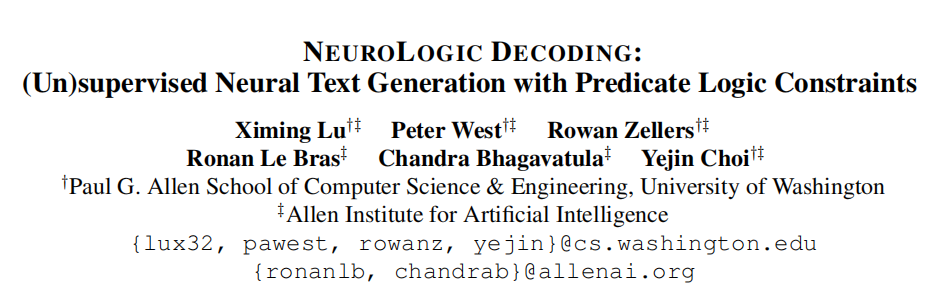
\includegraphics[width=4in]{figures/neural_decoding_info.png}
	        \caption{Paper information. \cite{lu_neurologic_2021} \blfootnote{[1] Ximing Lu, Peter West, Rowan Zellers, Ronan Le Bras, Chandra Bhagavatula, Yejin Choi. NeuroLogic Decoding: (Un)supervised Neural Text Generation with Predicate Logic Constraints. NAACL2021.}}
	        \label{fig:neural-decoding-info}
	    \end{figure}
    \end{frame}
    
    \begin{frame}
        \frametitle{\textbf{Task Definition}}
        \begin{figure}[!t]
            \centering
            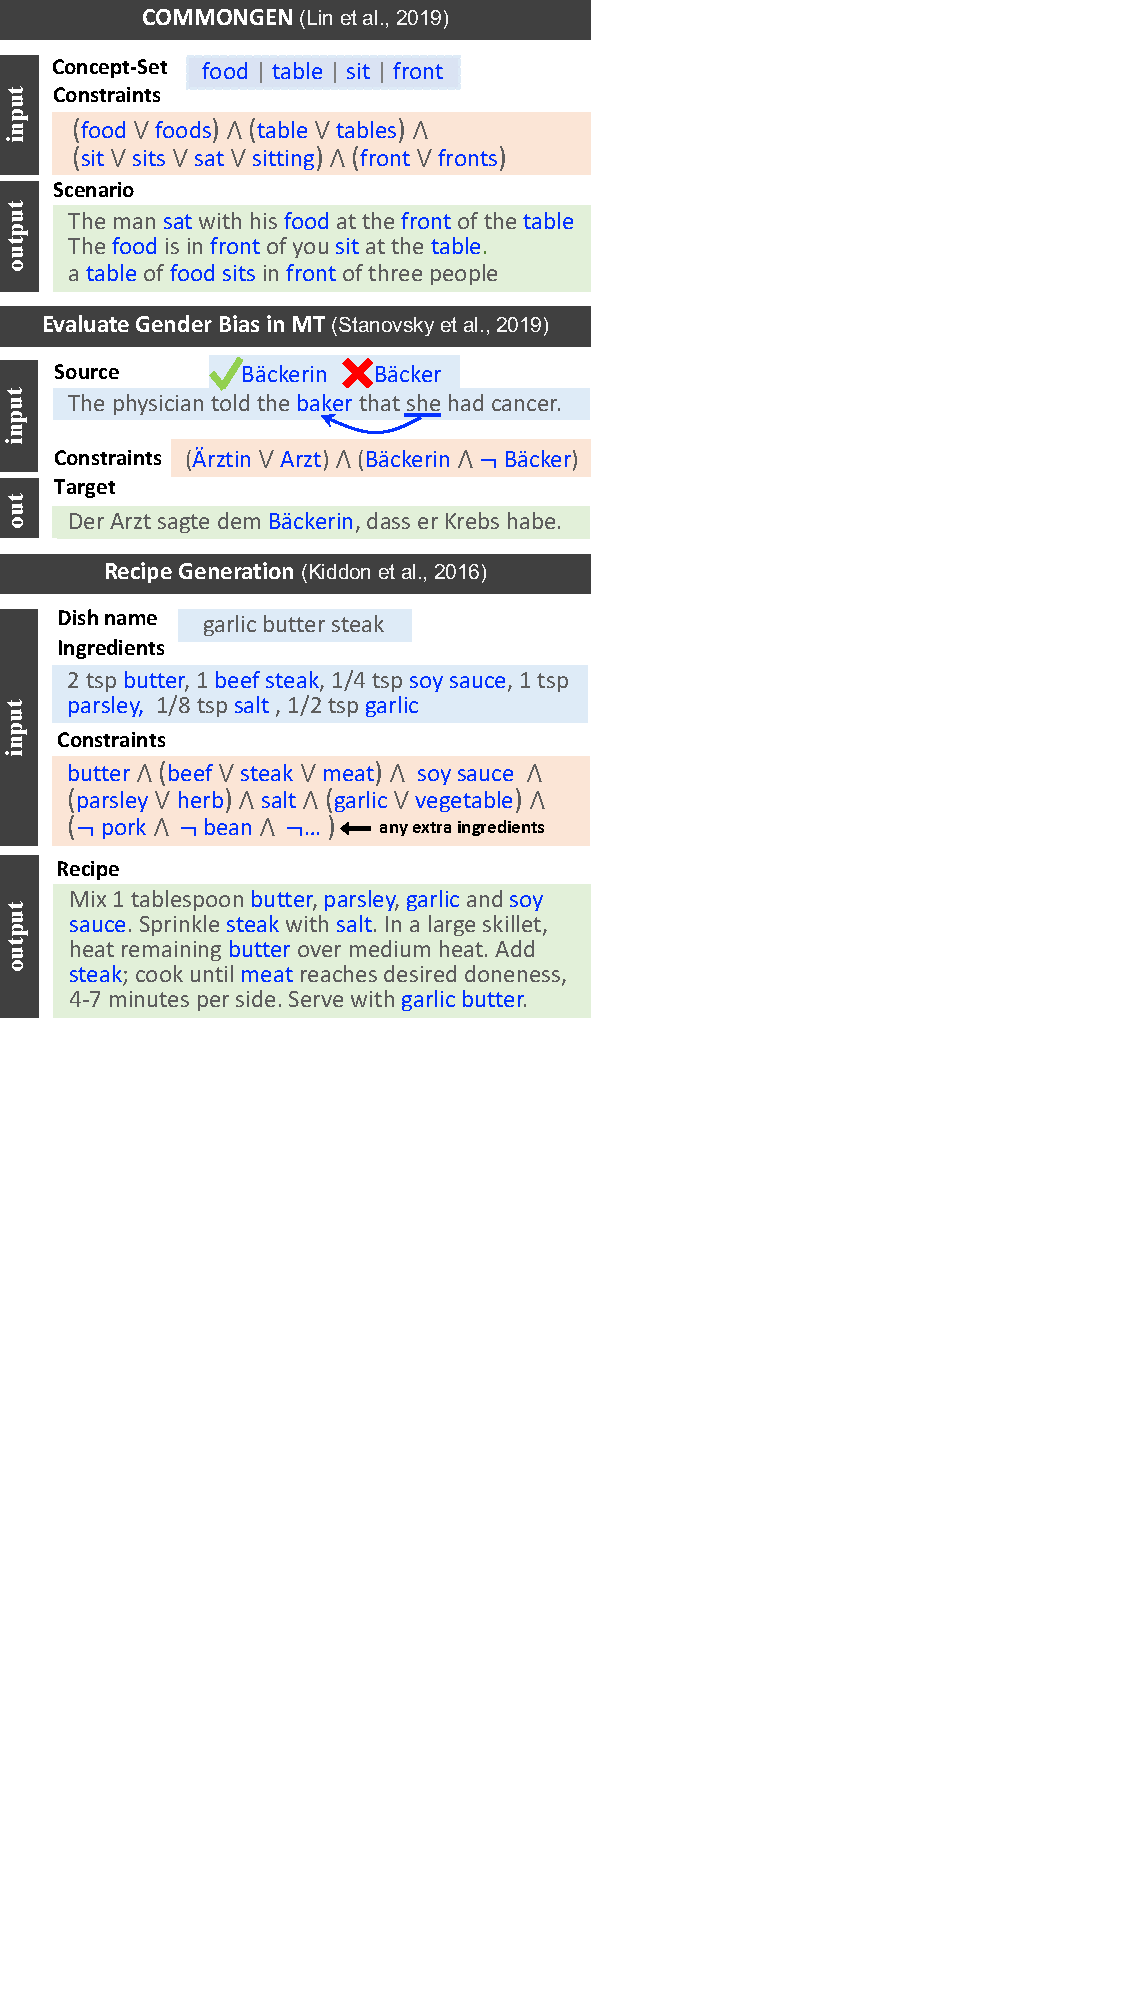
\includegraphics[width=1.5in]{figures/neural_decoding_task.pdf}
            \caption{An example for conditional text generation.}
            \label{fig:neural-decoding-task}
        \end{figure}
    \end{frame}
    
    \begin{frame}
        \frametitle{\textbf{Limitations of Previous Work}}
        \begin{itemize}
            \item \textbf{Finetuning LMs on a dataset of task-specific examples}. However, PLMs sturggle at learning to follow these constraints.
            \item \textbf{Mismatch caused by a fundamental under-specification of finetuning}. Improvements come from \textbf{constrained generation} or \textbf{learning the language style}? When increasing the finetuning data fed to GPT2 by \textbf{an order of magnitude}, constraint-satisfaction with standard beam search shows \textbf{only modest improvement}.
        \end{itemize}
    \end{frame}
    
    \begin{frame}
        \frametitle{\textbf{Contributions}}
        \begin{itemize}
            \item Proposing \textbf{\method{}}, which effectively enforces the satisfaction of given lexical constraints by controlling the decoding stage of sequence generation.
            \item  \textbf{Converting the hard logic constraints into a soft penalty term in the decoding objective}, and use a beam-based search to find approximately-optimal solutions.
            \item Empirical results demonstrate that \method{} ensures the satisfaction of given constraints while maintaining high generation quality, in turn leading to \textbf{new SOTA results in both the supervised and zero-shot setting}.
        \end{itemize}
    \end{frame}
    
    \begin{frame}
        \frametitle{\textbf{Prerequisite}}
        \begin{block}{\textbf{Predicate} $D(\textbf{a}, \textbf{y})$}
            Let us define a predicate $D(\textbf{a}, \textbf{y})$ to be a boolean function indicating the occurrence of key phrase $\textbf{a}$ in a sequence $\textbf{y}$, where \textbf{a} can be either unigram or multi-gram. $D(\textbf{a}, \textbf{y})$ will be true iff $\textbf{a}$ occurs in \textbf{y}.
            \begin{align*}
                &D(\textbf{a}, \textbf{y}) \equiv \exists \: i, \> \textbf{y}_{i:i+|\textbf{a}|} = \textbf{a}
            \end{align*}
            \methodshort{}  accepts lexical constraints in Conjunctive Normal Form:
            \begin{center}
                $\underbrace{\big(D_1 \lor D_2 \cdots \lor D_i \big)}_{C_1}\land \cdots \land \underbrace{\big(D_k \lor D_{k+1} \cdots \lor D_n \big)}_{C_m}$
            \end{center}
        \end{block}
        \begin{block}{\textbf{Notation}}
            \begin{itemize}
                \item Each individual constraint $D_{i}$ $\rightarrow$ a \emph{literal}.
                \item The disjunction of literals $\rightarrow$ a \emph{clause}, denoted as $C_{j}$.
            \end{itemize}
        \end{block}
    \end{frame}
    
    \begin{frame}
        \frametitle{\textbf{Prerequisite}}
        \begin{block}{\textbf{Objective}}
            The method seeks optimal sequences in which all clauses are satisfied:
            \begin{equation}
                \hat{\textbf{y}} {=} \arg\max_{\textbf{y} \in \mathcal{Y}}P_\theta(\textbf{y}|\textbf{x}) \hspace{1em}\textrm{where}\hspace{1em} \sum_{i=1}^{L} C_i{=}L
             \end{equation}
            By adding a high-cost penalty term for violated constrains, constrained optimization problem $\rightarrow$ unconstrained problem:
            \begin{align}
                \hat{\textbf{y}} = &\arg\max_{\textbf{y} \in \mathcal{Y}}P_\theta(\textbf{y}|\textbf{x}) - \lambda' \sum_{i=1}^{L} (1-C_i)
             \end{align}
            While exhaustive search is intractable, we use a beam-based search to find approximately optimal solutions for this objective.
        \end{block}
    \end{frame}
    
    \begin{frame}
        \frametitle{\textbf{Constraint States}}
        \begin{columns}[c]
            \column{.45\textwidth}
            \begin{figure}
                \centering
                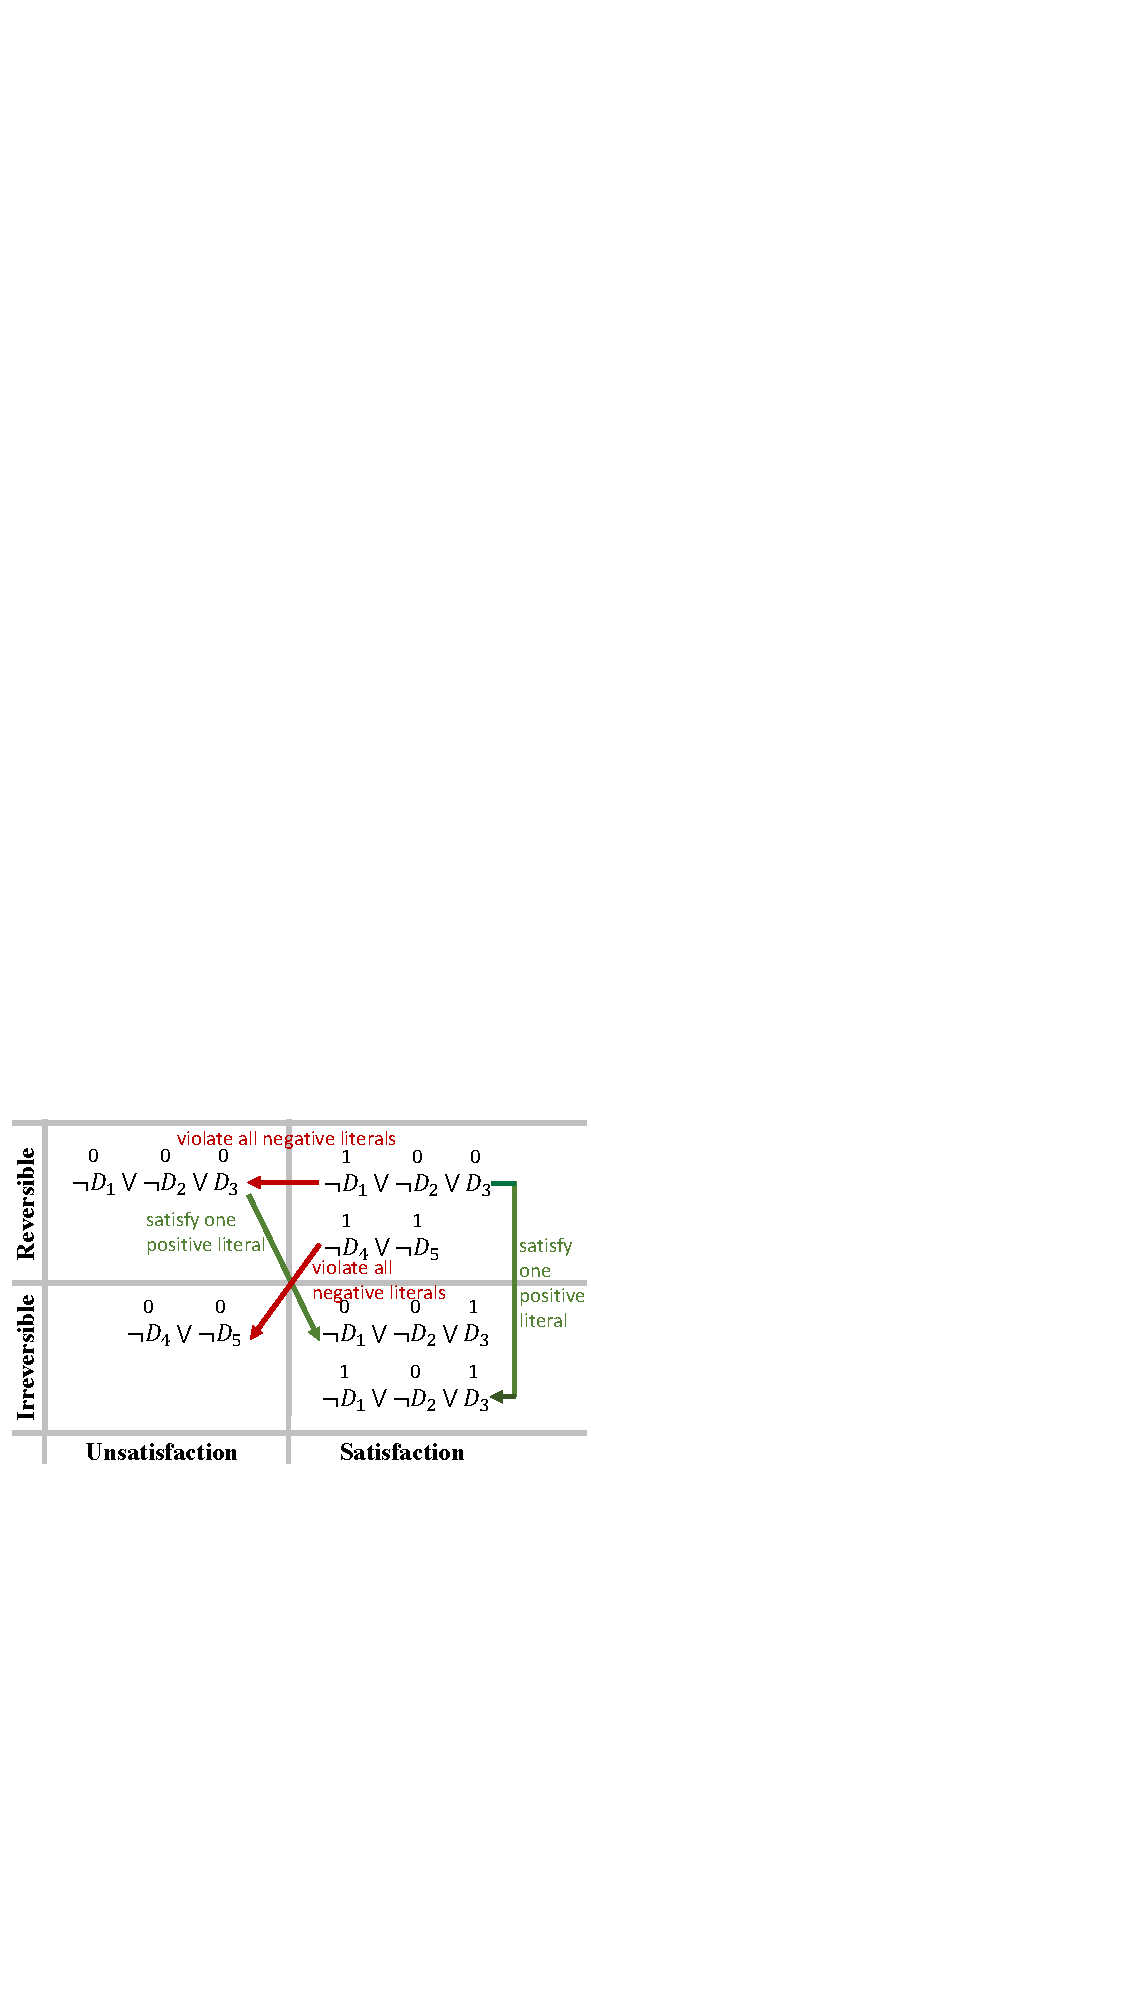
\includegraphics[width=1.3\textwidth]{figures/constrain_state.pdf}
                \caption{Clause states and possible transitions. $D_i$ and $\neg D_i$ denote positive and negative literal respectively}
                \label{fig:constrain_state}
            \end{figure}
            
            \column{.45\textwidth}
            \begin{description}
                \item[S1:] \textbf{reversible unsatisfaction}
                \item[S2:] \textbf{irreversible unsatisfaction}
                \item[S3:] \textbf{reversible satisfaction}
                \item[S4:] \textbf{irreversible satisfaction}
            \end{description}
        \end{columns}
    \end{frame}
    
    \begin{frame}
        \frametitle{\textbf{Tracking Constraint States}}
        \begin{block}{\textbf{Prefix Tries}}
            \begin{itemize}
                \item Prefix trie, $\mathcal{T}^{+}$ tracks \emph{unsatisfied positive} literals from all clauses in states S1 and S3.
                \item Prefix trie, $\mathcal{T}^{-}$  tracks \emph{satisfied negative} literals from all clauses in state S3.
            \end{itemize}
        \end{block}
        \begin{block}{\textbf{How Prefix Tries Changes}}
            \begin{itemize}
                \item a positive literal satisfied $\rightarrow$ its clause in state S1 or S3 henceforth irreversibly satisfied (state S4) $\rightarrow$ remove all literals of that clause from both tries and stop tracking.
                \item a negative literal violated $\rightarrow$ remove it from the trie $\mathcal{T}^{-}$ $\rightarrow$ switch back to S1 or S2 once all negative literals of a clause in state S3 has been removed.
            \end{itemize}
        \end{block}
    \end{frame}
    
    \begin{frame}
        \frametitle{\textbf{Algorithm}}
        \begin{block}{\textbf{High-level Intuition}}
            At at each time step, \methodshort{} selects generation hypotheses in consideration of both the objective function and the diversity of the partially satisfied constraints. We achieve such by 3 steps: \emph{pruning}, \emph{grouping}, and \emph{selecting}.
            \begin{description}
                \item[\textbf{Pruning Step:}] We first discard any $h$ with irreversible unsatisfied clause (state S2) to focus only on candidates that might satisfy all constraints.
                \item[\textbf{Grouping Step:}] Next, we select the beam from the pruned candidates.
                \item[\textbf{Selecting Step:}] To select best ones from each group, we first rank candidates within a group by score function:
            \end{description}
            \begin{equation}
                \textbf{s}= P_{\theta}\left(\textbf{y}_{t} \mid \textbf{y}_{<t}\right)+\lambda \cdot \max _{D\left(\textbf{a}_{\textbf{i}}, \textbf{y}\right) \atop \in \text {state} \textbf{S}1} \frac{\left|\hat{\textbf{a}}_{\textbf{i}}\right|}{\left|\textbf{a}_{\textbf{i}}\right|}
            \end{equation}            
        \end{block}
    \end{frame}
    
    \begin{frame}
        \frametitle{\textbf{Algorithm}}
        \begin{figure}
            \centering
            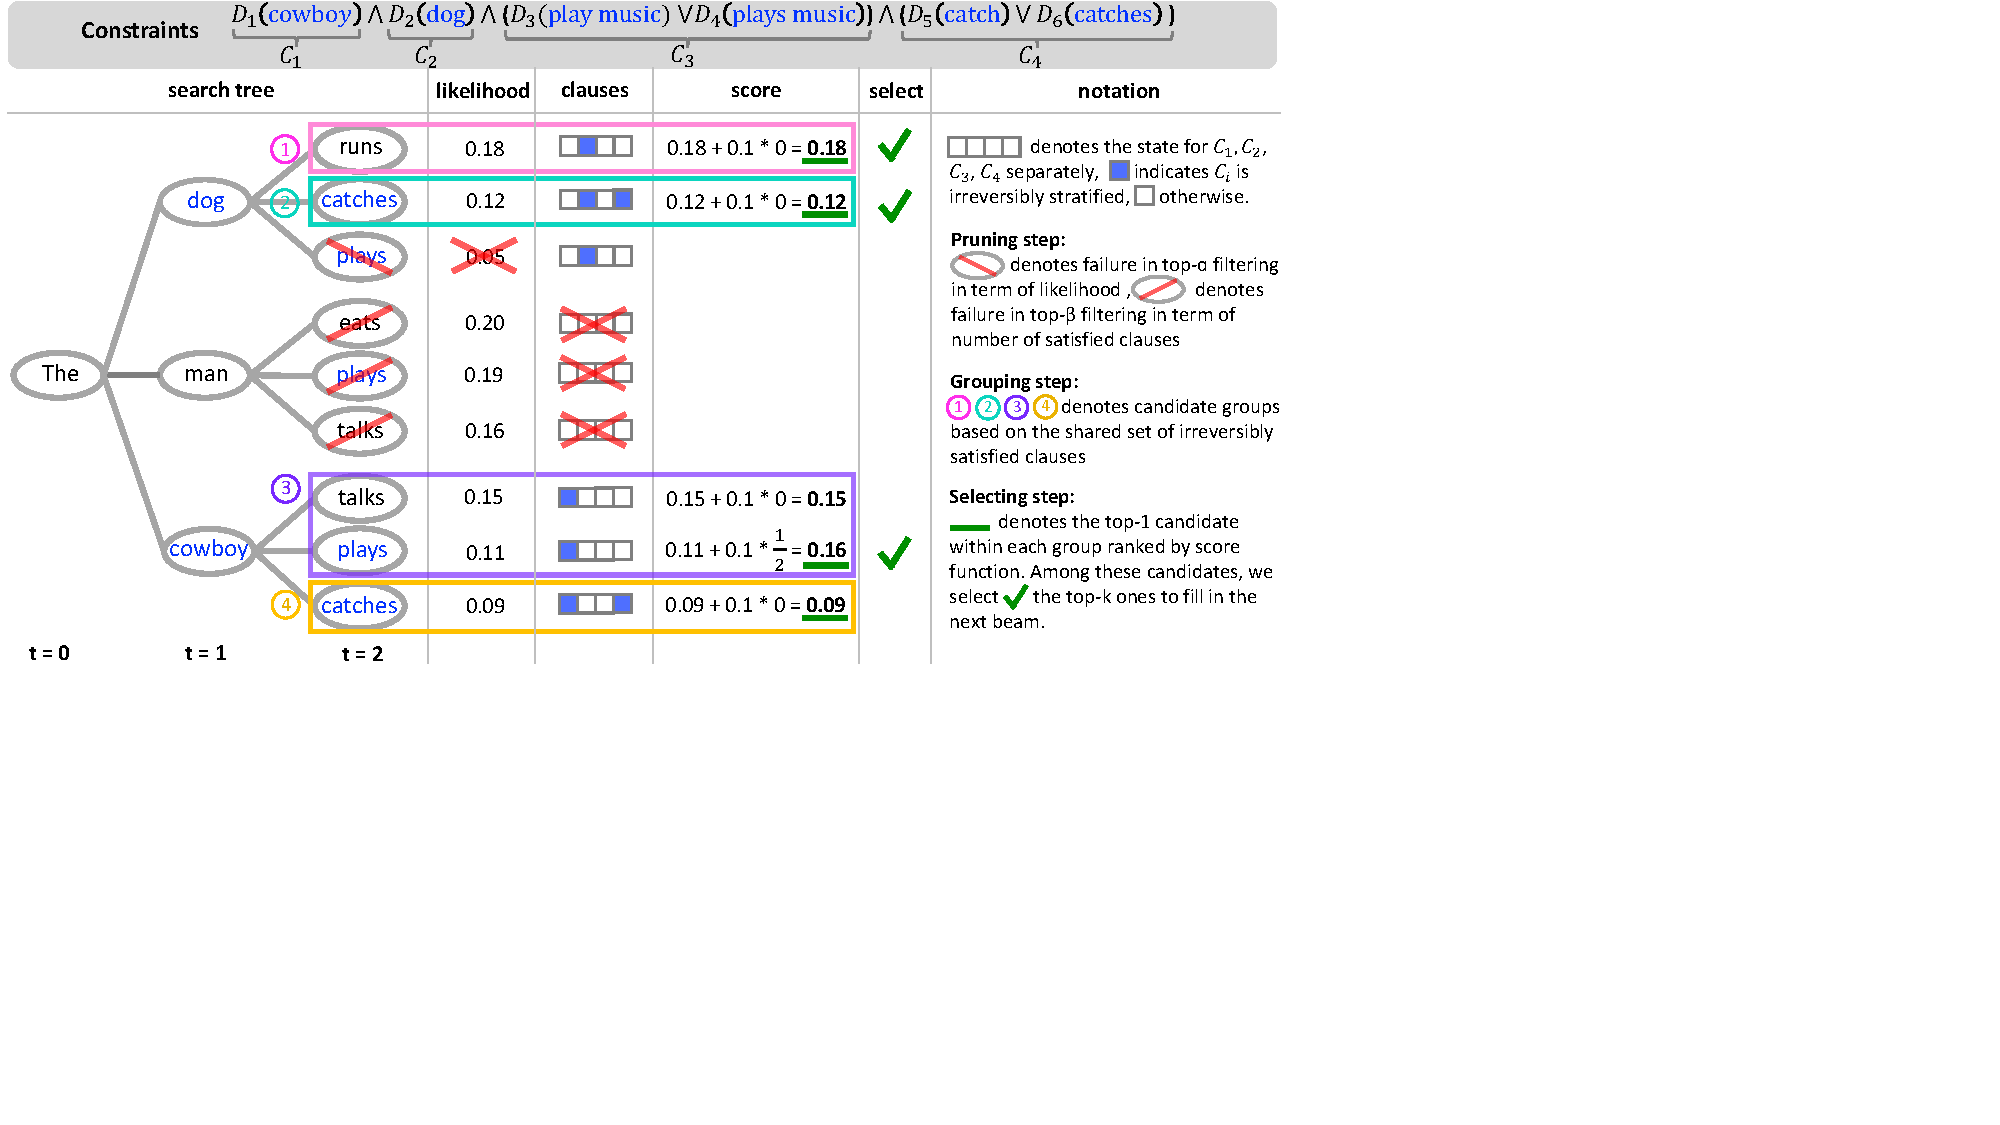
\includegraphics[width=4.2in]{figures/algorithm.pdf}
            \caption{Illustration of the \methodshort decoding procedure. In this example, $k=3$, $\alpha=8$, $\beta=2$, $\lambda=0.1$.}
            \label{fig:algorithm}
        \end{figure}
    \end{frame}
    
    \begin{frame}
        \frametitle{\textbf{Experiment I: Constrained Generation}}
        \begin{block}{\textbf{C{\small OMMON}G{\small EN} }\cite{lin-etal-2020-commongen} }
            C{\small OMMON}G{\small EN} is a benchmark dataset designed as a test of generative commonsense reasoning. Given a set of common concepts (e.g., dog, frisbee, catch, throw); the task is to generate a coherent sentence describing an everyday scenario using these concepts (e.g., ``a man throws a frisbee and his dog catches i'').
        \end{block}
        \blfootnote{[2] Bill Yuchen Lin, Wangchunshu Zhou, Ming Shen, Pei Zhou, Chandra Bhagavatula, Yejin Choi, Xiang Ren. CommonGen: A Constrained Text Generation Challenge for Generative Commonsense Reasoning. EMNLP2020, Findings.}
        \begin{block}{\textbf{Problem Formulation}}
            The input is an unordered set of $n$ concepts $\textbf{x} = \{a_1, a_2, \ldots , a_n\}$, where each concept $a_i$ is a common object (noun) or action (verb). The expected output is a simple, grammatical sentence $\textbf{y} \in \mathcal{Y}$ that describes a common scenario  using all given concepts in $\textbf{x}$ with correct morphological inflections. 
        \end{block}
    \end{frame}
    
    \begin{frame}
        \frametitle{\textbf{Results I: \methodshort{} vs Other Decoding Methods}}
        \begin{table}[!t]
            \setlength{\tabcolsep}{1pt}
            \resizebox{1\textwidth}{!}{
            \centering
            \begin{tabular}{p{2.7cm}| c|x{0.77cm} c|c|x{1.14cm} c|c}
                \toprule
                \rowcolor[gray]{0.90}\textbf{Decode Method}  &  \textbf{ROUGE-L} & \multicolumn{2}{c|}{\textbf{BLEU-3/4}}  & \textbf{METEOR} &\multicolumn{2}{c|}{\textbf{CIDEr}  \textbf{SPICE}} &\textbf{Coverage}\\ 
                \midrule
                Greedy Decoding &35.3 &25.2 & 16.7&25.8 &10.2 &24.4 & 80.3\\
                Top-k Sampling & 33.8& 22.5&14.4 &24.9 &9.2 &22.7 &79.4\\
                Top-p Sampling & 35.3& 25.0&16.5 &25.7 &10.2 &24.1 &80.1\\
                Beam Search & \underline{40.3} &\underline{34.2} & \underline{24.7}&\underline{27.6} &\underline{13.4} &\underline{27.1} & 82.2\\\midrule
                Hokamp and Liu  & 37.6 & 25.6& 16.8 & 25.9 & 11.1 & 25.1& 97.2\\
                Post and Vilar & 38.3&28.1 &18.6 &26.7 &11.8 &26.0 &\underline{97.4} \\
                Hu et al. &38.2 &27.8&18.4 &26.7 &11.7 &26.1 &\underline{97.4} \\
                \midrule
                \textsc{NeuroLogic} &\textbf{42.8}&\textbf{36.7}&\textbf{26.7}&\textbf{30.2}&\textbf{14.7}&\textbf{30.3}&\textbf{97.7}\\
                \bottomrule
            \end{tabular}}
            \caption{Performance of different decoding methods using supervised GPT2-L on the C{\scriptsize OMMON}G{\scriptsize EN} test set.}
            \label{tab:results1}
        \end{table}
    \end{frame}
    
    \begin{frame}
        \frametitle{\textbf{Results II: \methodshort{} across Different Supervised Models}}
        \begin{table}[!t]
            \setlength{\tabcolsep}{6pt}
            % \footnotesize
            \resizebox{1\textwidth}{!}{
            \centering
            \begin{tabular}{l|c|c c|c|c c|c}
                \toprule
                \rowcolor[gray]{0.90} \textbf{\hspace{8pt}Model} &  \multicolumn{1}{c|}{\textbf{ROUGE - L}} &  \multicolumn{2}{c|}{\textbf{BLEU - 3 \& 4}}  & \textbf{METEOR}  &\multicolumn{2}{c|}{\textbf{CIDEr} \hspace{15pt} \textbf{SPICE}} &\textbf{Coverage}\\ 
                \midrule
                GPT-2  %&19.2 $\rightarrow$ 21.0
                &40.3 $\rightarrow$ 42.8&34.2 $\rightarrow$ 36.7&24.7 $\rightarrow$ 26.7&27.6 $\rightarrow$ 30.2&13.4 $\rightarrow$ 14.7 &27.1 $\rightarrow$ 30.3&82.2 $\rightarrow$ 97.7\\
                BERT-Gen  %&20.9 $\rightarrow$ 22.0
                & 42.4 $\rightarrow$ 43.8&37.5 $\rightarrow$ 38.9&27.0 $\rightarrow$ 28.2&29.5 $\rightarrow$ 30.9&14.9 $\rightarrow$ 15.5&29.8 $\rightarrow$ \underline{31.4}&89.2 $\rightarrow$ 97.3\\
                UniLM %&23.3 $\rightarrow$ \textbf{24.3}
                &44.3 $\rightarrow$ \textbf{45.8}&40.6 $\rightarrow$ \textbf{42.8}&29.9 $\rightarrow$ \textbf{31.5}&30.1 $\rightarrow$ \textbf{31.7}&15.5 $\rightarrow$ \underline{16.6}&30.6 $\rightarrow$ \textbf{32.5}&90.5 $\rightarrow$ 97.8\\
                UniLM-v2  %&21.8 $\rightarrow$ 22.3
                &43.5 $\rightarrow$ 44.2&39.2 $\rightarrow$ 39.5&28.3 $\rightarrow$ 28.5&30.6 $\rightarrow$ \underline{31.3}&15.2 $\rightarrow$ \textbf{16.8}&30.8 $\rightarrow$ 31.1&92.8 $\rightarrow$ 97.9\\
                BART   %&23.0 $\rightarrow$ \underline{24.0}
                &43.3 $\rightarrow$ 44.7&39.9 $\rightarrow$ \underline{41.3}&29.1 $\rightarrow$ \underline{30.6}&30.4 $\rightarrow$ 31.0&15.2 $\rightarrow$ 15.9&30.6 $\rightarrow$ 31.0 &95.0 $\rightarrow$ \textbf{98.7}\\
                %T5-Base   %&17.6 $\rightarrow$ 20.1
                %&38.1 $\rightarrow$ 42.0&22.5 $\rightarrow$ 29.8&16.1 $\rightarrow$ 20.5&21.5 $\rightarrow$ 26.9&\hspace{1.7mm}9.0 $\rightarrow$ 12.2&22.4 $\rightarrow$ 26.9&70.7 $\rightarrow$ 97.7\\
                T5-Large  %&22.6 $\rightarrow$ 23.1
                &43.9 $\rightarrow$ \underline{44.8}&36.6 $\rightarrow$ 38.5&26.9 $\rightarrow$ 28.1&28.9 $\rightarrow$ 30.7&14.3 $\rightarrow$ 15.5&29.5 $\rightarrow$ 30.8&89.7 $\rightarrow$ \underline{98.5}\\
                \bottomrule
            \end{tabular}}
            \caption{Experimental results of different supervised models on the C{\scriptsize OMMON}G{\scriptsize EN} test set.}
            \label{tab:results2}
        \end{table}
    \end{frame}
    
    \begin{frame}
        \frametitle{\textbf{Results III: \methodshort{} with Unsupervised Models}}
        \begin{table}[!t]
            \resizebox{1\textwidth}{!}{
            \centering
            \begin{tabular}{c|l|c|c c|c|c c|c}
                \toprule
                \rowcolor[gray]{0.90} \textbf{Domain Adaption} & \textbf{Model}  &  \multicolumn{1}{c|}{\textbf{ROUGE -  L}} &  \multicolumn{2}{c|}{\textbf{BLEU - 3 \& 4}}  & \textbf{METEOR}  &\multicolumn{2}{c|}{\textbf{CIDEr}   \hspace{5pt} \textbf{SPICE}} &\textbf{Coverage}\\ 
                \midrule
                & GPT %&13.4 $\rightarrow$ 20.4 
                &26.7 $\rightarrow$ 41.3 &3.0 $\rightarrow$ 25.1 &1.1 $\rightarrow$ 15.9  & \hspace{1.7mm}9.2 $\rightarrow$ 28.8 &0.9 $\rightarrow$ 11.7 &8.0 $\rightarrow$ 29.7& 8.4 $\rightarrow$ \textbf{97.4} \\
                No & GPT-2 %&\hspace{1.7mm}7.1 $\rightarrow$ 20.1 
                &19.7 $\rightarrow$ \textbf{42.9} &4.1 $\rightarrow$ \underline{34.4} &1.5 $\rightarrow$ \underline{23.5} &11.2 $\rightarrow$ \underline{30.7} &0.4 $\rightarrow$ \underline{13.6} &7.1 $\rightarrow$ \underline{31.4} &8.3 $\rightarrow$ 96.0 \\
                \midrule
                Yes &GPT-2 %& 12.9 $\rightarrow$ \textbf{22.1}
                & 29.8 $\rightarrow$  \underline{42.4} & 9.5 $\rightarrow$ \textbf{36.1} & 4.0 $\rightarrow$ \textbf{25.1}  & 11.7 $\rightarrow$ \textbf{31.3} & 1.7 $\rightarrow$ \textbf{13.9} & 8.0 $\rightarrow$ \textbf{31.8} & 9.3 $\rightarrow$ \underline{96.1} \\
                \bottomrule
            \end{tabular}}
            \caption{Experimental results in zero-shot (unsupervised) setting on the C{\scriptsize OMMON}G{\scriptsize EN} test set with and without language domain adaption.}
            \label{tab:results3}
        \end{table}
    \end{frame}

    \begin{frame}
        \frametitle{\textbf{Results IV: Ablation}}
        \begin{figure}[!t]
            \centering
            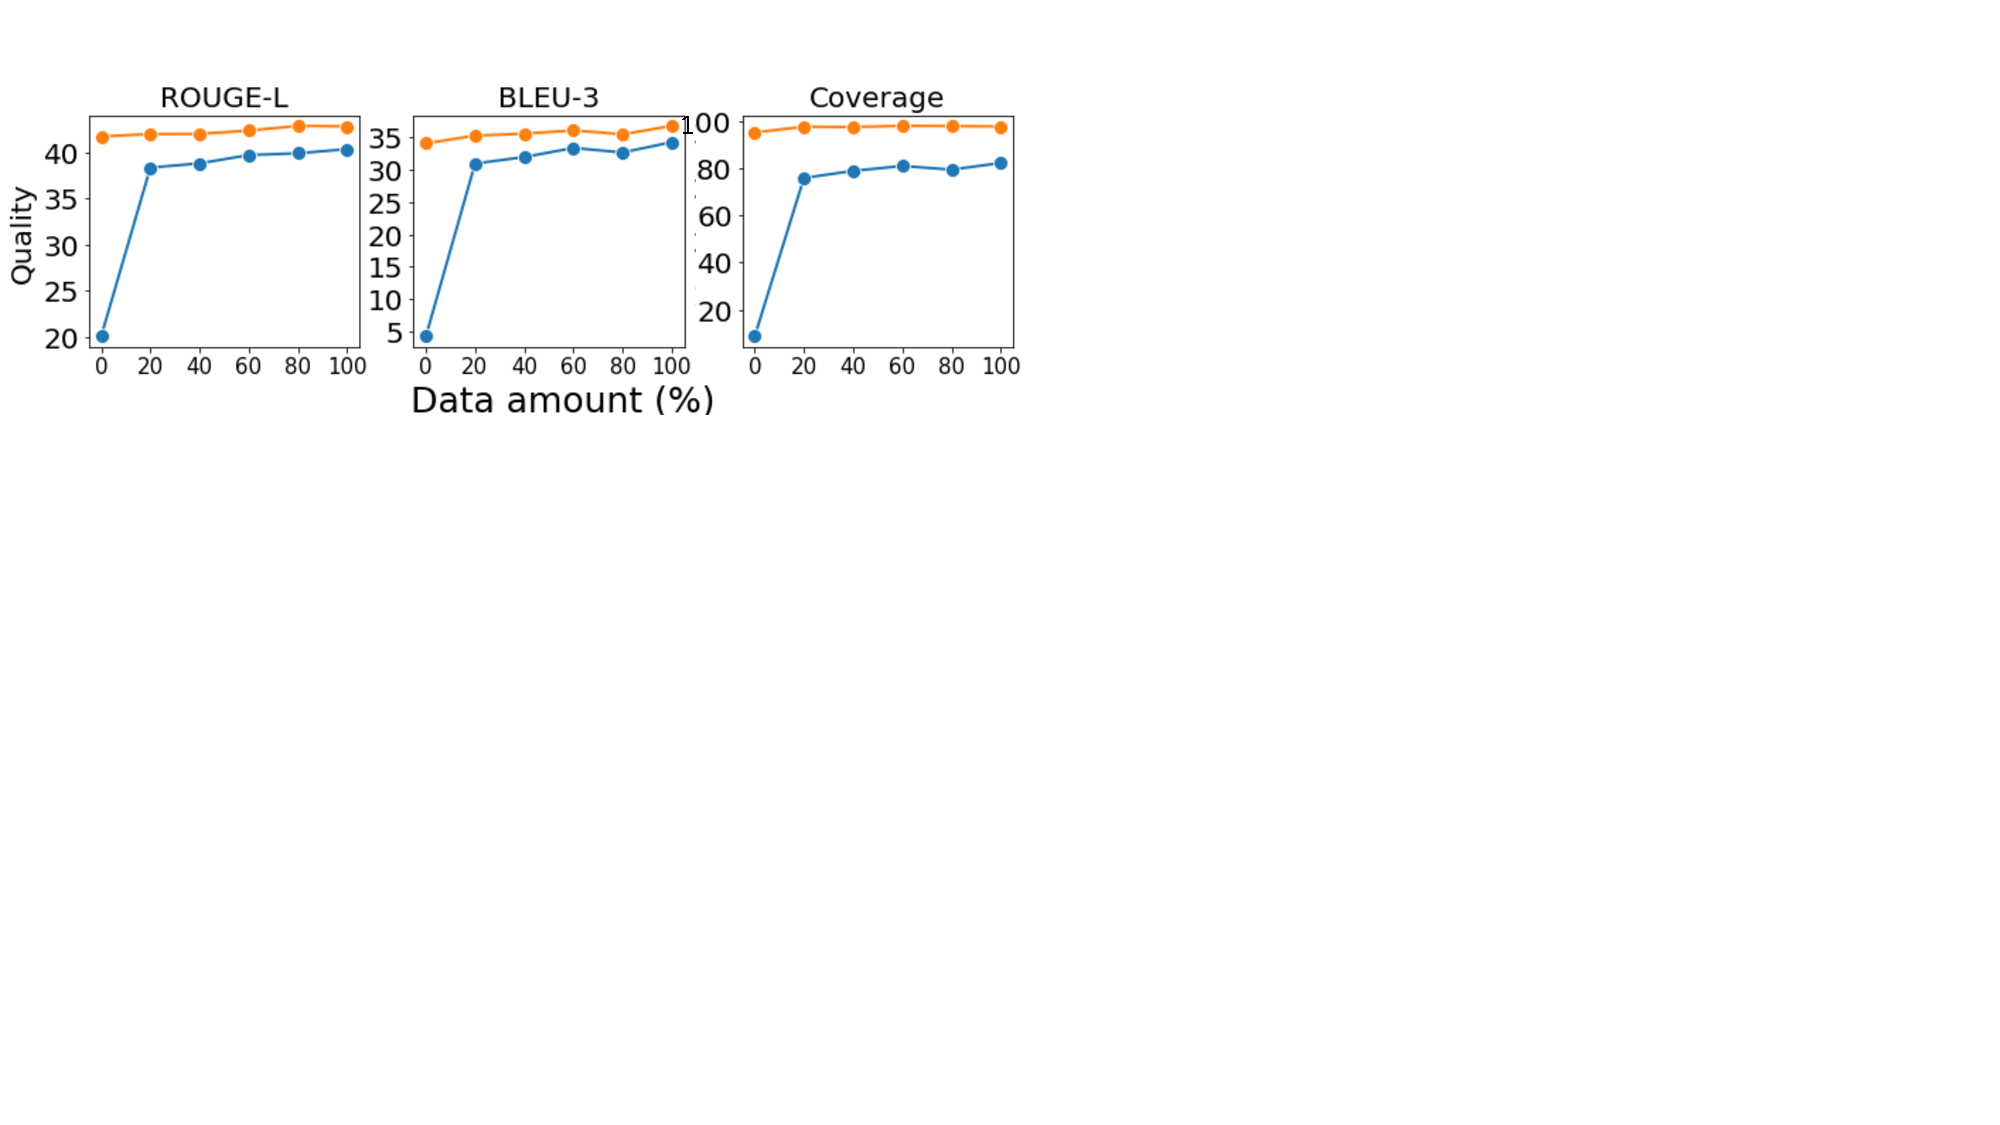
\includegraphics[width=3.1in]{figures/results4.pdf}
            \caption{Performance (y-axis) of supervised GPT2-L on C{\scriptsize OMMON}G{\scriptsize EN}, with a varying amount of training data for supervision (x-axis).}
            \label{fig:results4}
        \end{figure}
        \begin{figure}[!t]
            \centering
            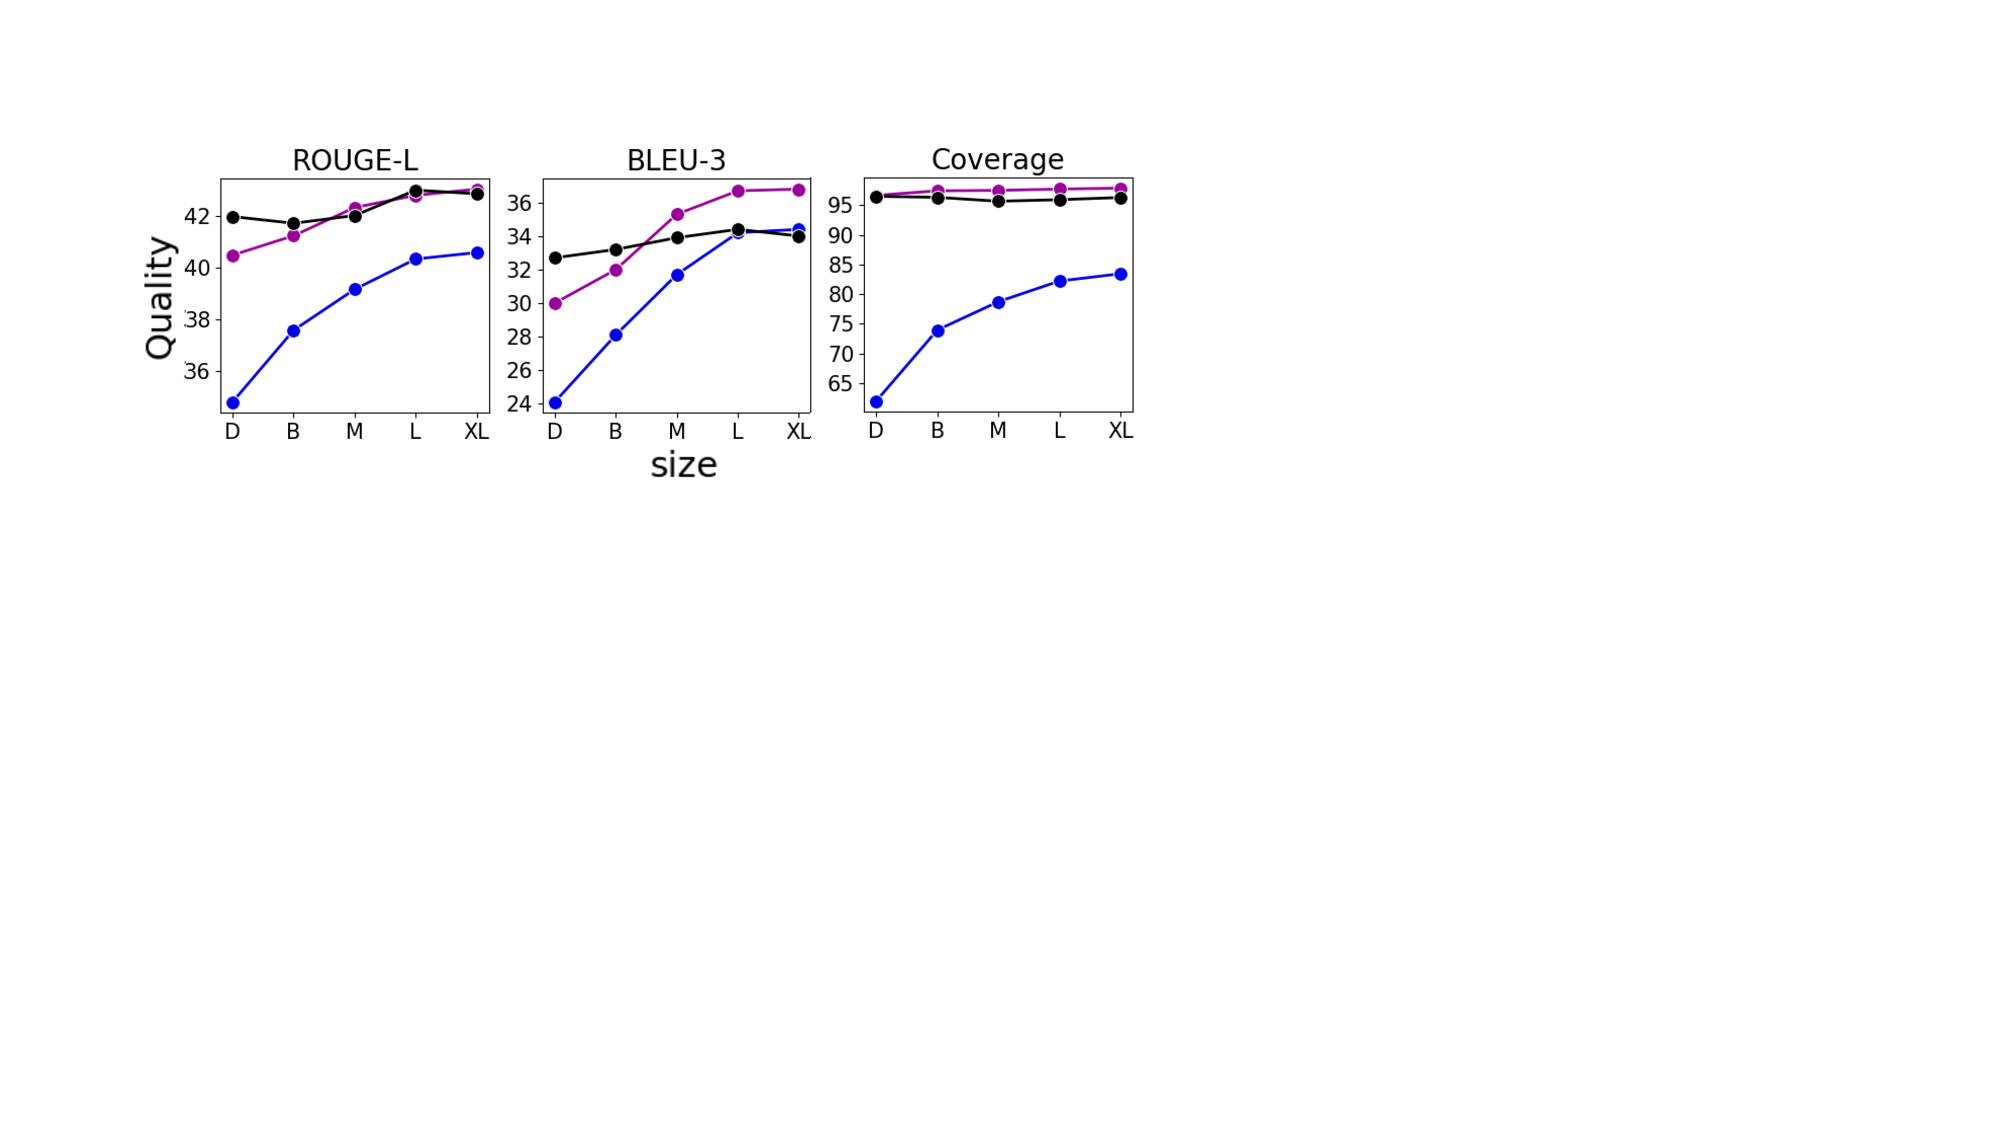
\includegraphics[width=3.1in]{figures/results5.pdf}
            \caption{Performance (y-axis) of GPT-2 with varying model sizes (x-axis).}
            \label{fig:results5}
        \end{figure}
    \end{frame}
    
    \begin{frame}
        \frametitle{\textbf{Experiment II Results: Recipe Generation}}
        \begin{table}[!t]
            \setlength{\tabcolsep}{1pt}
            \centering
            \resizebox{1\textwidth}{!}{
            \begin{tabular}{p{2.7cm}|c|x{0.77cm} c|c|c|c}
                \toprule
                \rowcolor[gray]{0.90}\textbf{Decode Method}  &  \textbf{ROUGE-L} &  \multicolumn{2}{c|}{\textbf{BLEU-3/4}}  & \textbf{METEOR} &\textbf{Coverage} &\textbf{Extra}\\ 
                \midrule
                Top-k Sampling  & 27.5& 15.2&9.5 &19.2  &84.8 &16.0\\
                Top-p Sampling &28.7 &\underline{17.6} &11.7 &19.4  &86.4 &15.4\\
                Beam Search &\underline{29.4} &17.4 & \underline{12.0}&\underline{19.7}  &86.5 &14.3\\\midrule
                Post and Vilar & 26.1&13.6 &8.8 &16.5  &\underline{89.6} &1.15 \\
                Hu et al &26.1 &13.6 &8.8 &16.5  &\underline{89.6} &\underline{1.13} \\
                \midrule
                \textsc{NeuroLogic} &\textbf{32.1}&\textbf{19.5}&\textbf{13.8}&\textbf{19.8}&\textbf{95.8}&\textbf{0.6}\\
                \bottomrule
           \end{tabular}}
           \caption{Experimental results of different decoding methods with RecipeGPT on the Recipe1M+ test set. Coverage indicates the average percentage of ingredients that are covered in the generated recipe, while Extra corresponds to the average ratio of hallucinated ingredients over the number of given ingredients.}
           \label{tab:exp2-results}
        \end{table}
    \end{frame}
 
     \begin{frame}
        \frametitle{\textbf{An Example Illustration}}
        \begin{figure}[!t]
            \centering
            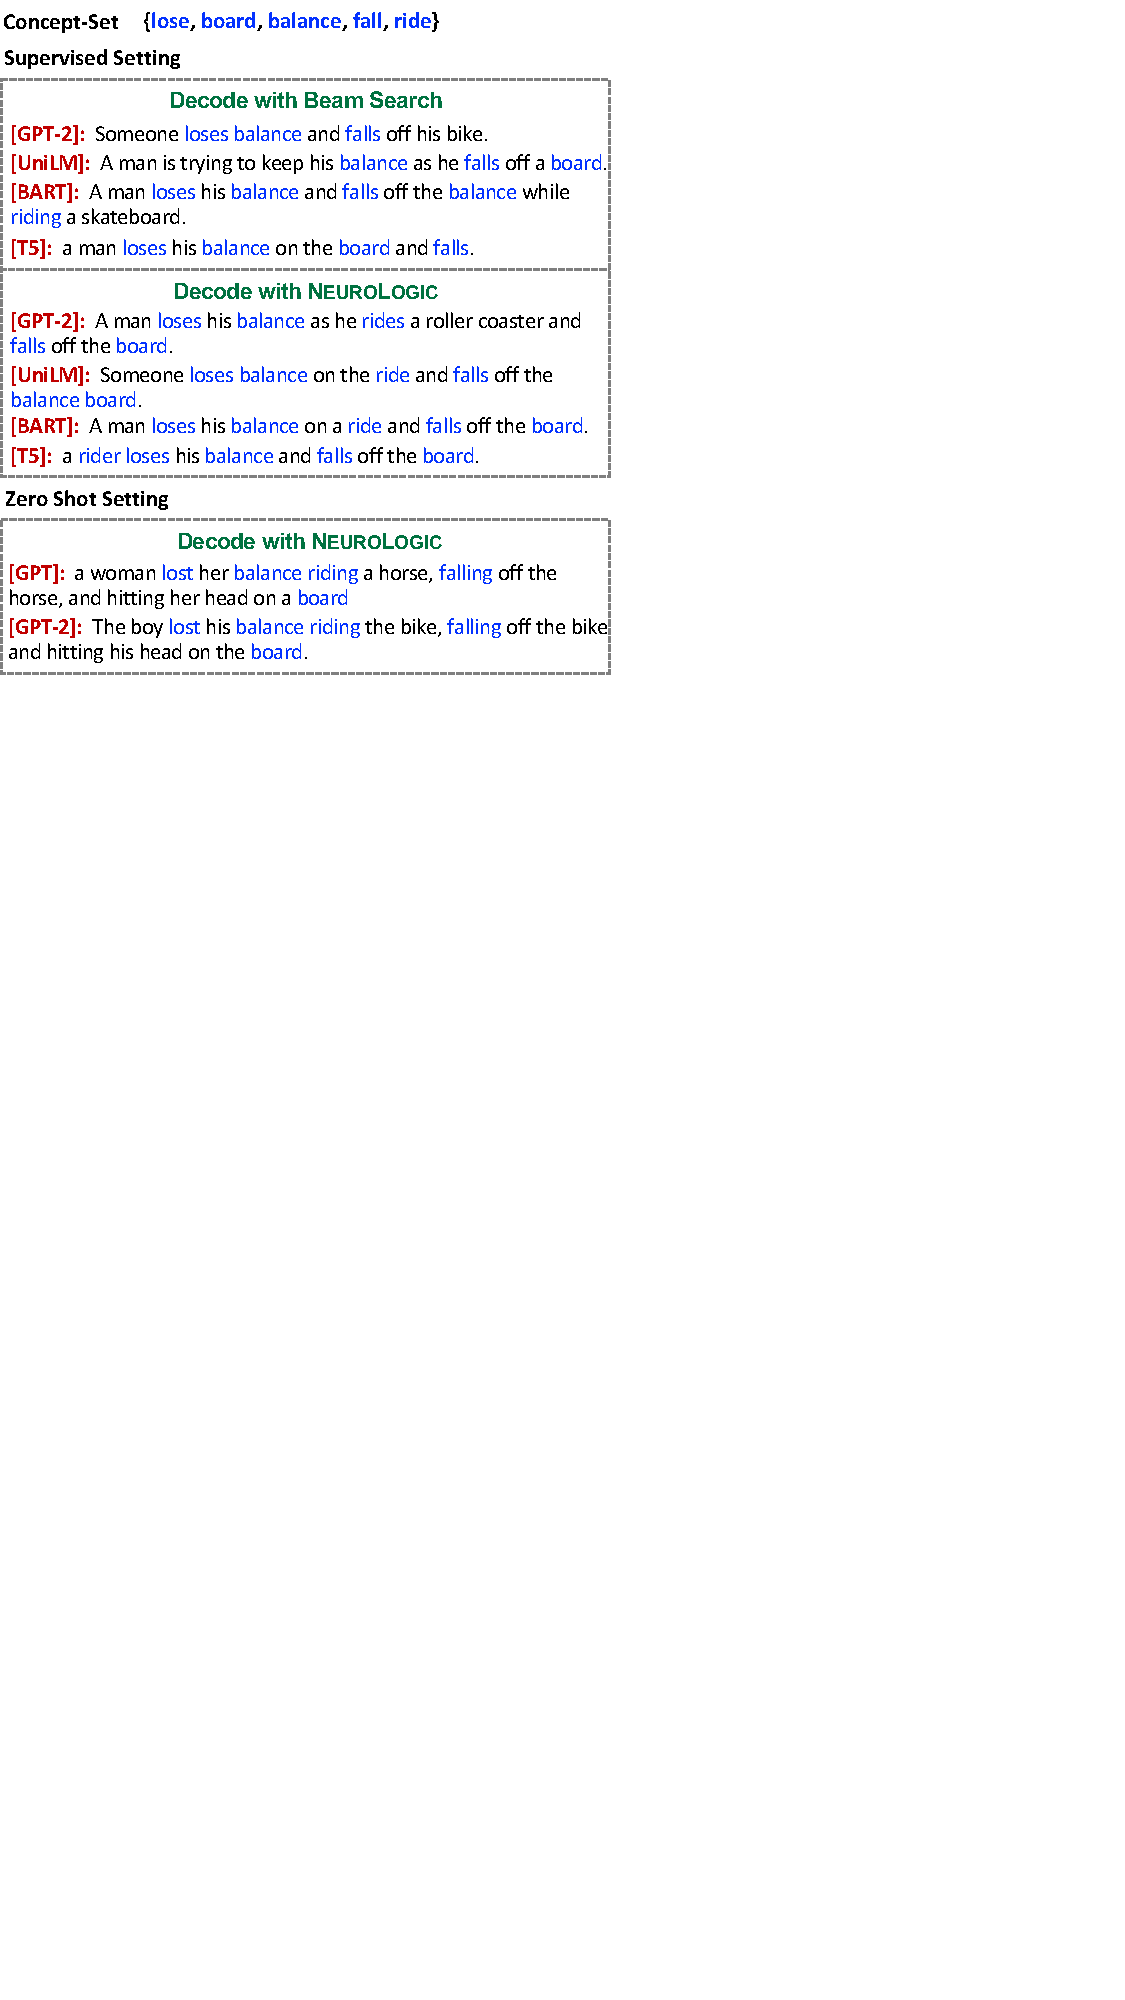
\includegraphics[width=2.3in]{figures/example1.pdf}
            \caption{Generated texts for the given concept-set.}
            \label{fig:examples1}
        \end{figure}
    \end{frame}
    
\section[Temporal Reasoning]{TEMPORAL REASONING}
    \begin{frame}
        \frametitle{\textbf{TEMPORAL REASONING}}
        \begin{figure}
            \centering
            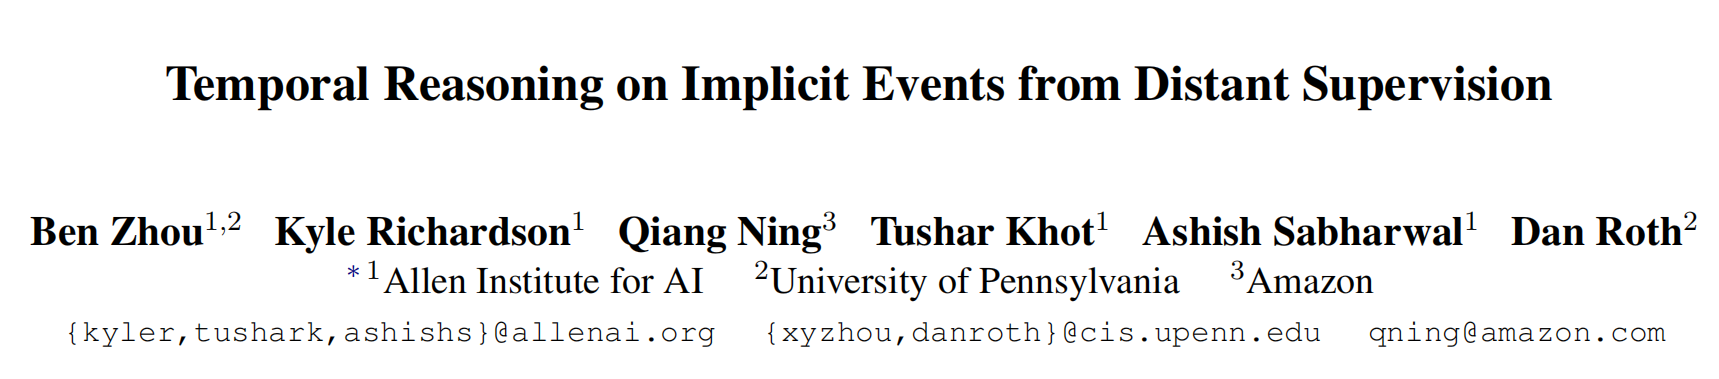
\includegraphics[width=4in]{figures/temporal_reasoning_info.png}
            \caption{Paper information. \cite{zhou_temporal_2021} \blfootnote{[3] Ben Zhou, Kyle Richardson, Qiang Ning, Tushar Khot, Ashish Sabharwal, D. Roth. Temporal Reasoning on Implicit Events from Distant Supervision. NAACL 2021.}}
            \label{fig:temporal-reasoning-info}
        \end{figure}
	\end{frame}
	
	\begin{frame}
	    \frametitle{\textbf{Task Definition}}
            \begin{figure}[!t]
                \centering
                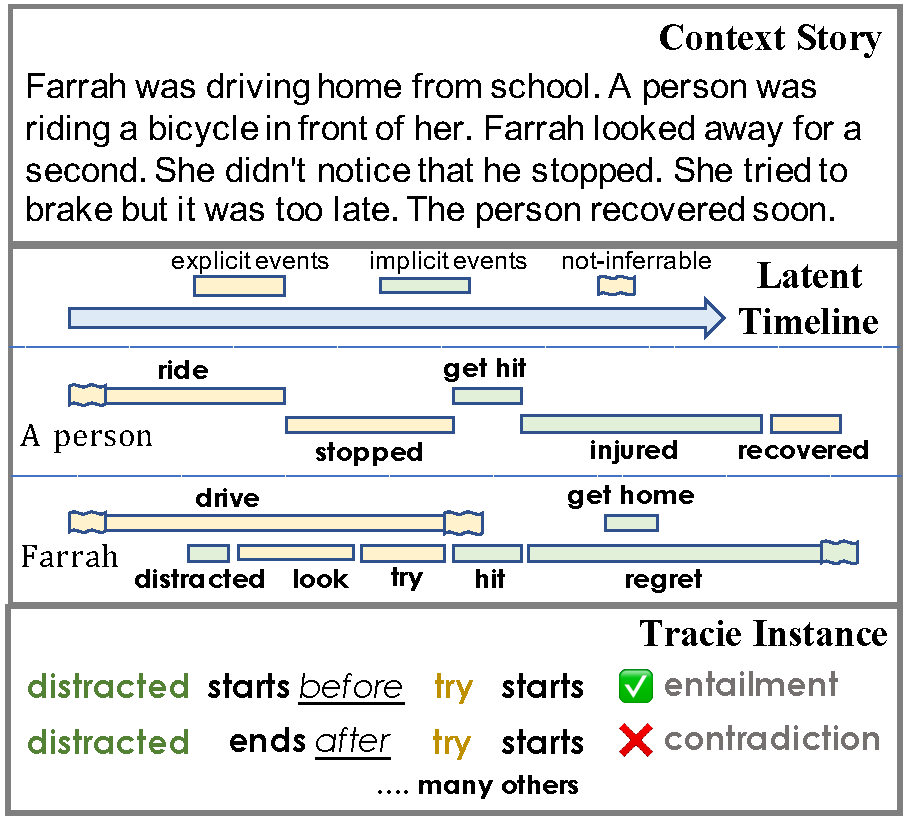
\includegraphics[width=2.7in]{figures/temporal_reasoning_task.pdf}
                \caption{The task focuses on temporal relations on implicit events in short stories. A story, its latent timeline, and example \datasetname{} instances from it. For simplicity, events are shortened to single verbs and the timeline is exaggerated.}
                \label{fig:temporal-reasoning-task}
            \end{figure}
	\end{frame}
	
	\begin{frame}
	    \frametitle{\textbf{Contributions}}
	    \begin{itemize}
	        \item A temporal relation dataset \datasetname{} focusing on \textbf{implicit events}.
	        \item A \textbf{distant supervision process} for temporal understanding of implicit events.
	        \item A \textbf{reasoning} model that makes end-time comparisons using predictions of start-time distances and durations.
	    \end{itemize}
	\end{frame}
	
	\begin{frame}
	    \frametitle{\textbf{The \datasetname{} Dataset}}
	    \begin{figure}
	        \centering
	        \resizebox{1\textwidth}{!}{
            \begin{tabular}{| p{7.8cm} | p{4.1cm} | l |}
                 \hline 
                 \multicolumn{1}{|c}{\textbf{Context Story} (Premise)} & \multicolumn{1}{c}{\textbf{Hypothesis}} & \multicolumn{1}{c|}{\textbf{Inference Label}} \\ \hline
                 \emph{Tom needed to get braces. He was afraid of them. The dentist assured him everything would be fine. Tom had them on for a while. Once \hlgray{removed} he felt it was worth it.} & Tom avoids foods he can't eat with braces \hl{\texttt{starts}} \hlcyan{\texttt{before}} \hlgray{the braces are removed}. & \texttt{entailment} \\ \hline 
                 \emph{We were all \hlgray{watching Spongebob as a family}. It is a kid's show but all really enjoyed it. This one episode was especially funny for the adults. It has humor in it that is funny for kids and adults. It is something we can all watch...} & The adults laughed at the jokes \hl{\texttt{ends}} \hlcyan{\texttt{before}} \hlgray{we watch Spongebob as a family} & \texttt{contradiction} \\ \hline 
                 \emph{I was throwing the baseball with my son. He threw one past me that landed in the lake. \hlgray{I reached in to get the ball}. I lost my balance and fell in. I got the ball and a bath all in one shot!} & The ball was in the boys hand \hl{\texttt{starts}} \hlcyan{\texttt{after}} \hlgray{he reached for the ball} & \texttt{contradiction} \\ \hline
            \end{tabular}}
	        \caption{Example \datasetname{} instances. The \hl{\textbf{comparator}}  $l \in $\{\texttt{starts},\texttt{ends}\} and \hlcyan{\textbf{relation}} $r \in$\{\texttt{before},\texttt{after}\} in each hypothesis are highlighted, in addition to the corresponding \hlgray{explicit event} from the story.}
	        \label{fig:TRACIE-data}
	    \end{figure}
	\end{frame}

	\begin{frame}
	    \frametitle{\textbf{The \datasetname{} Dataset}}
	    \begin{figure}
	        \centering
	        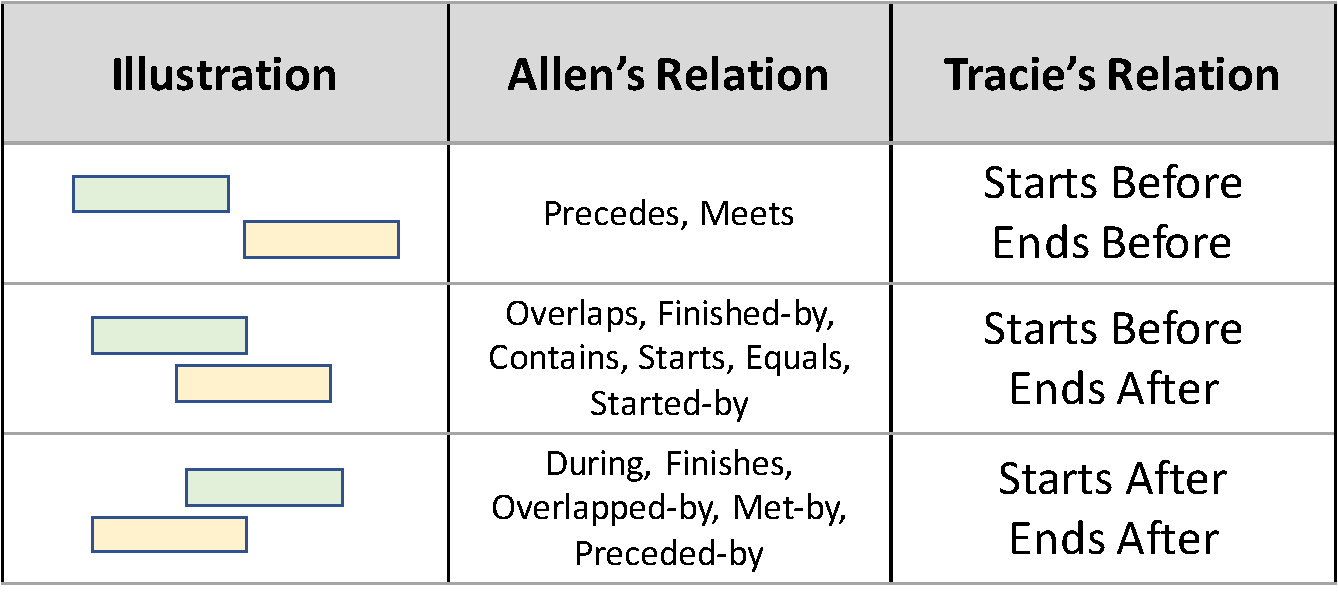
\includegraphics[width=4in]{figures/TRACIE_label.pdf}
	        \caption{\datasetname{}'s label definition and its relation to Allen's interval algebra, with a graph illustration between an \textcolor{implicit-color}{implicit event} and an \textcolor{explicit-color}{explicit event}.}
	        \label{fig:TRACIE-label}
	    \end{figure}
	\end{frame}
	
	\begin{frame}
	    \frametitle{\textbf{Implicit Event Generation}}
	    \begin{enumerate}
	        \item We randomly sample short stories from the ROCStories dataset \cite{mostafazadeh2016corpus}.
	        \item For each story, one annotator writes 5 implicit event phrases that are not explicitly mentioned by the given story, but are inferable and relevant.
	        \item The annotator additionally rewrites two explicit events closest to the implicit event's start and end time, respectively.
	        \item With these two events, we can build two \datasetname{} instances (minus the \textit{temporal-relation}) per implicit event, which accounts for 10 instances in total per story.
	    \end{enumerate}
	    \blfootnote{[4] Nasrin Mostafazadeh, Nathanael Chambers, Xiaodong He, Devi Parikh, Dhruv Batra, Lucy Vanderwende, Pushmeet Kohli, and James Allen. A Corpus and Evaluation Framework for Deeper Understanding of Commonsense Stories. NAACL2016.}
	\end{frame}
	
	\begin{frame}
	    \frametitle{\textbf{Pattern-Based Pre-Training}}
	    \begin{block}{High-level Intuition}
	        we believe that it is more efficient to build a model that learns the prior knowledge needed for the task with distant signals and only subsequently learns the task definition through a small training set.
	    \end{block}
	\end{frame}

	\begin{frame}
	    \frametitle{\textbf{Distant Supervision Collection}}
	    \begin{figure}
	        \centering
	        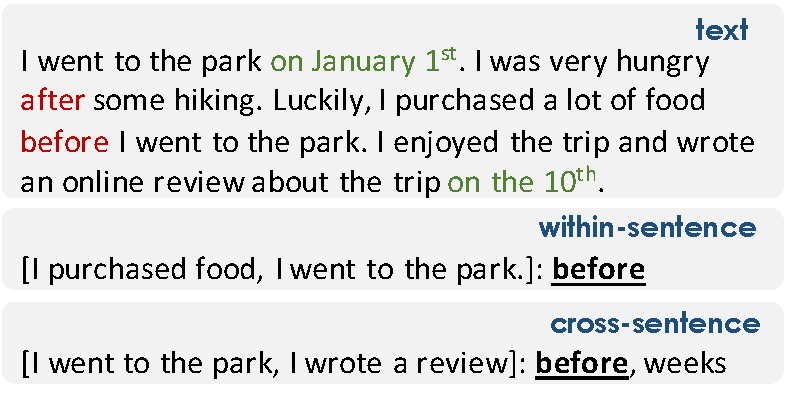
\includegraphics[width=3.6in]{figures/fig-extraction-short.pdf}
	        \caption{Extraction for start-time comparisons applied to an example paragraph.}
            \label{fig:extraction-example}
	    \end{figure}
	    We describe the sources of distant supervision signals with the goal of understanding the relative order between two events’ start times as well as the relative distance between them.
	\end{frame}

	\begin{frame}
	    \frametitle{\textbf{Supervision Instances Construction}}
	    \begin{enumerate}
	        \item Each instance comprises an event pair, a temporal relation, and an estimation on the temporal difference between the two start times.
	        \item Each event is a phrase constructed by taking all relevant arguments of the predicate verb in the SRL parses.
	        \item We represent the differences between the two start times as one of seven coarse temporal units: \{$\leq$minutes, hours, days, weeks, months, years, $\geq$decades\}.
	        \item In addition to the event pairs, we randomly sample sentences within the paragraph to use as the context that better defines the events.
	    \end{enumerate}
	\end{frame}

	\begin{frame}
	    \frametitle{\textbf{Pattern-Based Temporal Model (\modelpattern)}}
	    \begin{block}{\textbf{Data Format}}
	        \begin{description}
	            \item[Input sequences] \keywordCode{event:[EventA] starts[Relation][EventB].story:[Paragraph].}
	            \item [Output sequences] \keywordCode{answer:[Label][Distance]}.	            
	        \end{description}
	    \end{block}
	    \begin{block}{\textbf{\modelpattern}}
	        \begin{itemize}
	            \item We use a pre-trained sequence-to-sequence model as our base model and additionally pre-train this model using the data collected.
	            \item \modelpattern{} serves as new set of \emph{temporally-aware} model weights that can be used in place of existing pre-trained models and fine-tuned on \datasetname{}.
	        \end{itemize}
	    \end{block}
	\end{frame}
	
	\begin{frame}
	    \frametitle{\textbf{\datasetname{} Task Formulation}}
	    \begin{figure}[t]
	        \centering
	        \resizebox{1\textwidth}{!}{
	        \begin{tabular}{c  l}
	            \hline 
	            \textbf{comparator $l$} & \multicolumn{1}{c}{\textbf{relation  }\textbf{$r_{l}$$(\text{\hlgray{e$_{1}$}},\text{\hlgray{e$_{2}$}})$=}} \\ 
	            \hline 
	            \hl{\textbf{ends}} & {$
	            \begin{cases}
	            \hlcyan{\textbf{before}} & \text{if }\mathbf{end}_{1} < \mathbf{start}_{2} \\
	            \hlcyan{\textbf{after}} &\textit{otherwise}
	            \end{cases}
	            $}
	            \\ 
	            \hl{\textbf{starts}} & {$
	            \begin{cases}
	            \hlcyan{\textbf{before}} & \text{if }\mathbf{start}_{1} < \mathbf{start}_{2} \\
	            \hlcyan{\textbf{after}} &\textit{otherwise}
	            \end{cases}
	            $}
	            \\ 
            \end{tabular}}
	        \caption{Decomposition of the relation functions that solve \datasetname{} instances (equal timepoints ignored).}
            \label{fig:sym_func}
        \end{figure}
	\end{frame}

    \begin{frame}
        \frametitle{\textbf{Neural-symbolic Model}}
	    \begin{block}{\textbf{Two Modules}}
	        \begin{itemize}
	            \item Distance function: $\mathrm{dist}(e_i, e_j) = \mathbf{start}_{i} - \mathbf{start}_{j}$.
	            \item Duration function: $\mathrm{dur}(e_{j}) = \mathbf{duration}_{j}$.
	        \end{itemize}
	    \end{block}
	    By exploiting the rule that an end point $\mathbf{end}_{j}$ can be computed as $\mathbf{end}_{j} = \mathbf{start}_{j} + \mathbf{duration}_{j}$, we can, for example, decompose the relation $r_{ends}(e_{1},e_{2}) = \textbf{before}$ (i.e., \emph{$e_{1}$ ends before $e_{2}$}) in terms of our two modules as follows via simple algebraic manipulation:
	    \begin{align*}
	        &r_{ends}(e_{1},e_{2}) = \textbf{before} \\
	        &\Leftrightarrow\ \mathbf{end_1} < \mathbf{start_{2}}  \\
	        &\Leftrightarrow\ \mathbf{start_{1}} + \mathbf{duration_{1}} < \mathbf{start_{2}} \\ &\Leftrightarrow\ \big( \mathbf{start_{1}} - \mathbf{start_{2}}\big) + \mathbf{duration_{1}} < 0 \\
	        &\Leftrightarrow\ \mathrm{dist}(e_1, e_2)+ \mathrm{dur}(e_1) < 0
	   \end{align*}
	\end{frame}	
	
	\begin{frame}
	    \frametitle{\textbf{Distance Estimation}}
	    \begin{itemize}
	        \item We use the output from \modelpattern{} to approximate the function $\mathrm{dist}(\cdot)$.
	        \item Following the sequence formulation of \modelpattern{}, we replace \keywordCode{[EventA]} with the textual description of $e_1$, \keywordCode{[EventB]} with the textual description of $e_2$, and \keywordCode{[Paragraph]} with the context (premise), and fix \keywordCode{[Relation]} to be \textit{before}. By taking the values of the vocabulary indices corresponding to ``positive'' and ``negative'' from the logits of \keywordCode{[Label]} and applying a $\mathrm{softmax}$ operation, we get $P_{\textrm{before}}$ and $P_{\textrm{after}}$. These are the probability of $e_1$ starting before and after $e_2$, respectively, and are used to define the vector $\vb{p}=[P_{\textrm{before}}, P_{\textrm{after}}]$.
	        \item Similarly, we apply $\mathrm{softmax}$ to the logits of \keywordCode{[Distance]} over the 7 words representing the temporal units to obtain 7 values that approximate the probabilities of the distance between two events' start times being closest to each temporal unit. We place the 7 values in temporal units' increasing order in vector $\vb{d}$. To represent $|\mathbf{start_1}-\mathbf{start_2}|$ with a single value, we dot product the probabilities with an incremental constant vector $\vb{c}=[0,1,2,3,4,5,6]$. To get the direction, we apply the $\mathrm{tanh}$ function to the difference between the probabilities in $\vb{p}$.
	    \end{itemize}
	\end{frame}	
	
	\begin{frame}
	    \frametitle{\textbf{Duration Estimation}}
	    \begin{itemize}
	        \item To obtain a model to estimate $\mathrm{dur}(\cdot)$, we pre-train a sequence-to-sequence model with the duration data from \cite{zhou-etal-2020-temporal}.
	        \item The data contains over 1 million events with their corresponding duration values.
	        \item We map each instance to an input sequence \keywordCode{event:[Event]story:[Story]} and a corresponding output sequence \keywordCode{answer:[Value]}.
	    \end{itemize}

	    \blfootnote{[5] Ben Zhou, Qiang Ning, Daniel Khashabi, and Dan Roth. Temporal Common Sense Acquisition with Minimal Supervision. ACL2020. \\}
	\end{frame}
	

	
	\begin{frame}
	    \frametitle{\textbf{Computation and Learning}}
            \begin{columns}[c]
                \column{0.5\textwidth}
                    \begin{figure}
            	        \centering
            	        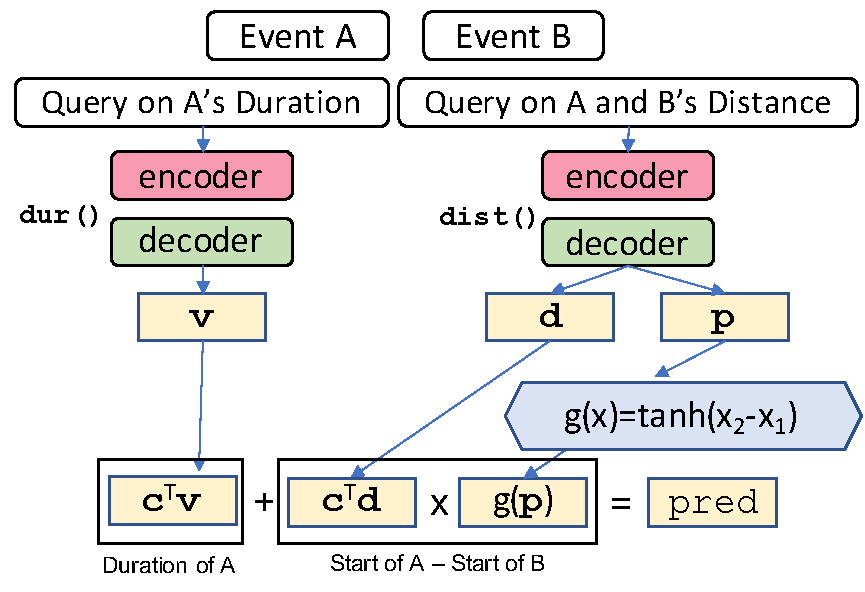
\includegraphics[width=1.0\textwidth]{figures/movel_v2.pdf}
            	        \caption{A schematic overview of \modelsymbolic{} to compare event $A$'s end time with event $B$'s start time via modular predictions about $A$'s duration and distance from $B$ and their symbolic combination (bottom).}
            	        \label{fig:model-overview}
        	        \end{figure}
        	    \column{0.5\textwidth}
        	        \begin{small}
                    	\begin{equation} 
            	            \label{eq-start-module}
            	            \begin{split}
                    	        \mathrm{dist}(\cdot) &= \mathbf{start_1} - \mathbf{start_2} \\
                    	        &= \vb{c}^T\vb{d}*\mathrm{tanh}(\textrm{INT}_{max}*(\mathbf{p}_2-\mathbf{p}_1)) \\
            	            \end{split}
            	        \end{equation}        	             
        	        \end{small}
        	        \begin{small}
             	        \begin{equation}
            	            \mathrm{dur}(\cdot) = \mathbf{duration_1} = \vb{c}^T\vb{v}
            	        \end{equation}       	        
        	        \end{small}

            \end{columns}
	\end{frame}
	
	\begin{frame}
	    \frametitle{\textbf{Results I: I.I.D Setting}}
	    \begin{table}[t]
	        \centering
	        \resizebox{0.7\textwidth}{!}{
                \begin{tabular}{l|ccc|c}
                    \toprule 
                    System  &\ Start\ \ &\ End\ \ &\ All\ &\ Story\ \\ 
                    \cmidrule(lr){1-1}                              \cmidrule(lr){2-2} \cmidrule(lr){3-3} \cmidrule(lr){4-4} \cmidrule(lr){5-5}
                    Majority & 57.3 & 69.8 & 64.1 & 18.1 \\
                    BiLSTM & 53.7 & 63.5 & 59.1 & 10.9\\ \cdashline{1-5}
                    Roberta-Large & 78.5 & 78.3 & 78.4 & 26.1\\
                    T5-3B & 79.4 & 77.4 & 78.3 & 26.9 \\
                    \midrule
                    BaseLM (T5-large) & 75.5 & 75.4 & 75.4 & 22.6 \\
                    BaseLM-MATRES & 76.7 & 76.3 & 76.5 & 25.3 \\ \cdashline{1-5}
                    \modelpattern{} (ours) & 81.4 & 77.5 & 79.3 & 31.0 \\
                    \modelsymbolic{} (ours) & \textbf{82.1} & \textbf{79.4} & \textbf{80.6} & \textbf{32.0} \\ \cmidrule(lr){1-5}
                    \modelzeroshot{} & 77.0 & 73.1 & 74.9 & 21.6 \\
                    \bottomrule 
                \end{tabular}}
            \caption{Performance on \datasetname{}, best numbers in \textbf{bold}. BaseLM is T5-large; Story is the percentage of story-wide exact match; Majority is based on the comparator and temporal-relation distribution; Zeroshot uses no TRACIE instance as supervision.}
            \label{tab:performance-iid-main}
        \end{table}
	\end{frame}
	
	\begin{frame}
	    \frametitle{\textbf{Results II: Uniform-prior Training Setting}}
	    \begin{table}[t]
	        \centering
	        \resizebox{0.7\textwidth}{!}{
	        \begin{tabular}{l|ccc|c}
                \toprule 
                System                                     &\ Start\ \ &\ End\ \ &\ All\ &\ $\Delta$All\ \\ 
                \cmidrule(lr){1-1}                              \cmidrule(lr){2-2} \cmidrule(lr){3-3} \cmidrule(lr){4-4} \cmidrule(lr){5-5}
                Random & 50.0 & 50.0 & 50.0 & -14.1 \\
                BiLSTM & 50.5 & 51.2 & 50.9 &  -8.2 \\ \cdashline{1-5}
                Roberta-Large & 75.1 & 68.1 & 71.3 & -7.1 \\ 
                T5-3B & 72.8 & 68.6 & 70.5 & -7.8 \\
                \midrule
                BaseLM (T5-large) & 68.1 & 67.8 & 67.9 & -7.5 \\
                BaseLM-MATRES & 76.3 & 69.9 & 72.8 & -3.7 \\ \cdashline{1-5}
                \modelpattern{} (ours) & 80.6 & 73.2 & 76.6 & -2.7\\
                \modelsymbolic{} (ours) & \textbf{81.2} & \textbf{77.0} & \textbf{78.9} & -1.7 \\ \cmidrule(lr){1-5}
                \modelzeroshot{} & 77.0 & 73.1 & 74.9 & \textbf{0.0} \\
                \bottomrule 
            \end{tabular}}
            \caption{Performance on \datasetname{}a uniform-prior training setting. $\Delta$All compares the difference with Table~\ref{tab:performance-iid-main}; Majority is equivalent to random guessing.}
            \label{tab:performance-iid-balanced}
        \end{table}
	\end{frame}
	
	\begin{frame}
	    \frametitle{\textbf{Results III: MATRES for Explicit Events}}
	    \begin{table}[t]
            \centering
            \resizebox{0.7\textwidth}{!}{
            \begin{tabular}{l|c|c|c|c}
                \toprule 
                System                                     & OT-NS & OT & OT-MS & PT \\ 
                \cmidrule(lr){1-1}                              \cmidrule(lr){2-2} \cmidrule(lr){3-3} \cmidrule(lr){4-4} \cmidrule(lr){5-5}
                Wang et.al.(2020) & 85.9 & - & - & - \\
                BaseLM & 86.0 & 87.5 & 77.4 & 69.0  \\
                \modelpattern{} & 87.3 & 89.6 & 86.1 & 75.1 \\
                \bottomrule 
            \end{tabular}}
            \caption{Performance on MATRES\cite{WCZR20} is not strictly comparable with the rest.}
            \vspace{-1em}
            \label{tab:performance-matres}
        \end{table}
        \blfootnote{[6] Haoyu Wang, Muhao Chen, Hongming Zhang, and Dan Roth. Joint constrained learning for event-event relation extraction. EMNLP2020. \\}
	\end{frame}
	
	\begin{frame}
	    \frametitle{\textbf{Results IV: Ablation}}
	    \begin{table}[t]
            \centering
            \resizebox{0.8\textwidth}{!}{
            \begin{tabular}{c|c|c|c|c}
                \toprule 
                Sys.                                    & BaseLM & \modelpattern{} & \modelsymbolic{}& Human\\ 
                \cmidrule(lr){1-1} \cmidrule(lr){2-2} \cmidrule(lr){3-3} \cmidrule(lr){4-4} \cmidrule(lr){5-5}
                Acc. & 52.6 & 72.2 & 75.3 & 82.5\\
                \bottomrule 
            \end{tabular}}
            \caption{Performance on \textit{no-story} \datasetname{} under the uniform-prior training setting.}
            \vspace{-1em}
            \label{tab:performance-ablation-hyponly}
        \end{table}
        \begin{table}[t]
            \centering
            \resizebox{0.8\textwidth}{!}{
            \begin{tabular}{c|c|c|c}
                \toprule 
                Sys.                                    & \modelpattern{} & cross-sentence & within-sentence \\ 
                \cmidrule(lr){1-1} \cmidrule(lr){2-2} \cmidrule(lr){3-3} \cmidrule(lr){4-4}
                Acc. & 80.6 & 79.9 & 63.7\\
                \bottomrule 
            \end{tabular}}
            \caption{Comparison of pre-training data sources on \datasetname{}'s start time prediction accuracy, under the uniform-prior training setting.}
            \vspace{-1em}
            \label{tab:performance-ablation-source}
        \end{table}
	\end{frame}

\section[COMET-ATOMIC]{(\textsc{Comet}-)\textsc{Atomic}${^{20}_{20}}$}

	\begin{frame}
	    \frametitle{(\textbf{\textsc{Comet}-)\textsc{Atomic}${^{20}_{20}}$}}
	    \begin{figure}[!t]
	        \centering
	        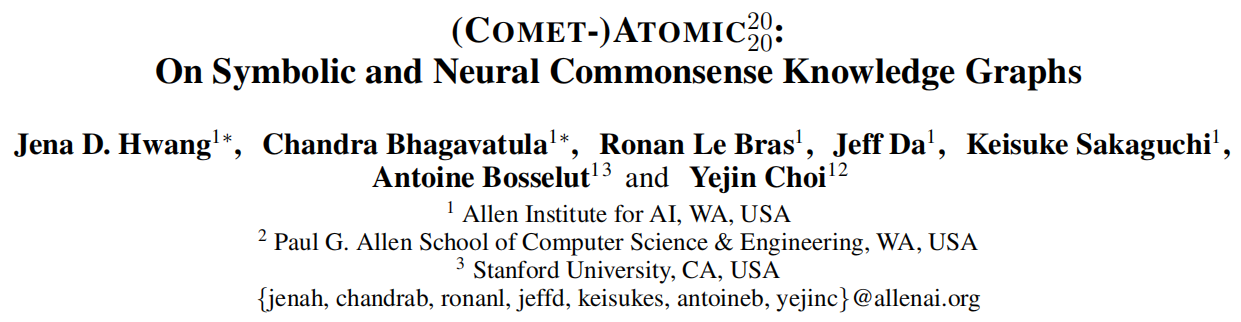
\includegraphics[width=4in]{figures/comet_info.png}
	        \caption{Paper information. \cite{hwang_comet-_2021} \blfootnote{[7] Jena D. Hwang, Chandra Bhagavatula, Ronan Le Bras, Jeff Da, Keisuke Sakaguchi, Antoine Bosselut, Yejin Choi. COMET-ATOMIC 2020: On Symbolic and Neural Commonsense Knowledge Graphs. AAAI 2021.}}
	        \label{fig:comet_info}
	    \end{figure}
    \end{frame}
    
    \begin{frame}
        \frametitle{\textbf{Motivation}}
        \begin{itemize}
            \item A new paradigm of language models as knowledge bases has emerged. In this setting, language models are \textbf{prompted} with natural language prefixes or questions, and they express knowledge through language generation.
            \item \textit{Does scaling up language models actually endow them with commonsense knowledge?} They perform better when evaluated on knowledge bases that \textbf{prioritize ontological relations} and whose examples resemble language-like assertions (e.g., mango \IsA{} fruit).
            \item Prior work has also shown that training language models on knowledge graph tuples leads them to learn to \textbf{express their implicit knowledge directly}, allowing them to provide commonsense knowledge on-demand.
        \end{itemize}
    \end{frame}
    
    \begin{frame}
        \frametitle{\textbf{Contributions}}
        \begin{itemize}
            \item We present \atomicTT{}---\textbf{a new commonsense knowledge graph} covering social, physical, and eventive aspects of everyday inferential knowledge.
            \item We compare \atomicTT{} with other prominent CSKBs head-to-head and show that our new \textit{symbolic} knowledge graph is \textbf{more accurate than any current CSKB}.
            \item We show that our new \textit{neural} knowledge model \comet{}-\atomicTT{} \textbf{successfully transfers \atomicTT{}'s declarative knowledge} to beat \gpttt{}, the largest pre-trained language model, in spite of using ~400x fewer parameters.
        \end{itemize}
    \end{frame}
    
    \begin{frame}
        \frametitle{\textbf{Comparisons of Three CSKGs}}
        \begin{figure}
            \centering
            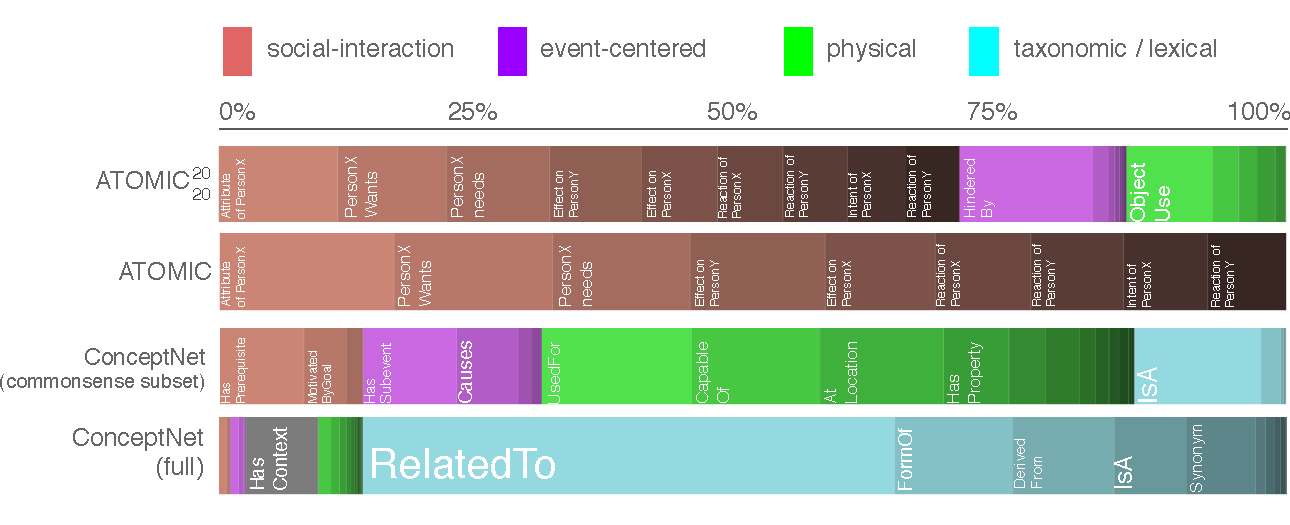
\includegraphics[width=4in]{figures/atomic2020_v3.pdf}
            \caption{\atomicTT{} tuple count distribution compared to \atomic and \conceptnet, either its commonsense subset or the full set.}
            \label{fig:tuple_distribution}
        \end{figure}
    \end{frame}   
    
    \begin{frame}
        \frametitle{\textbf{\atomicTT{} Illustration}}
        \begin{figure}
            \centering
            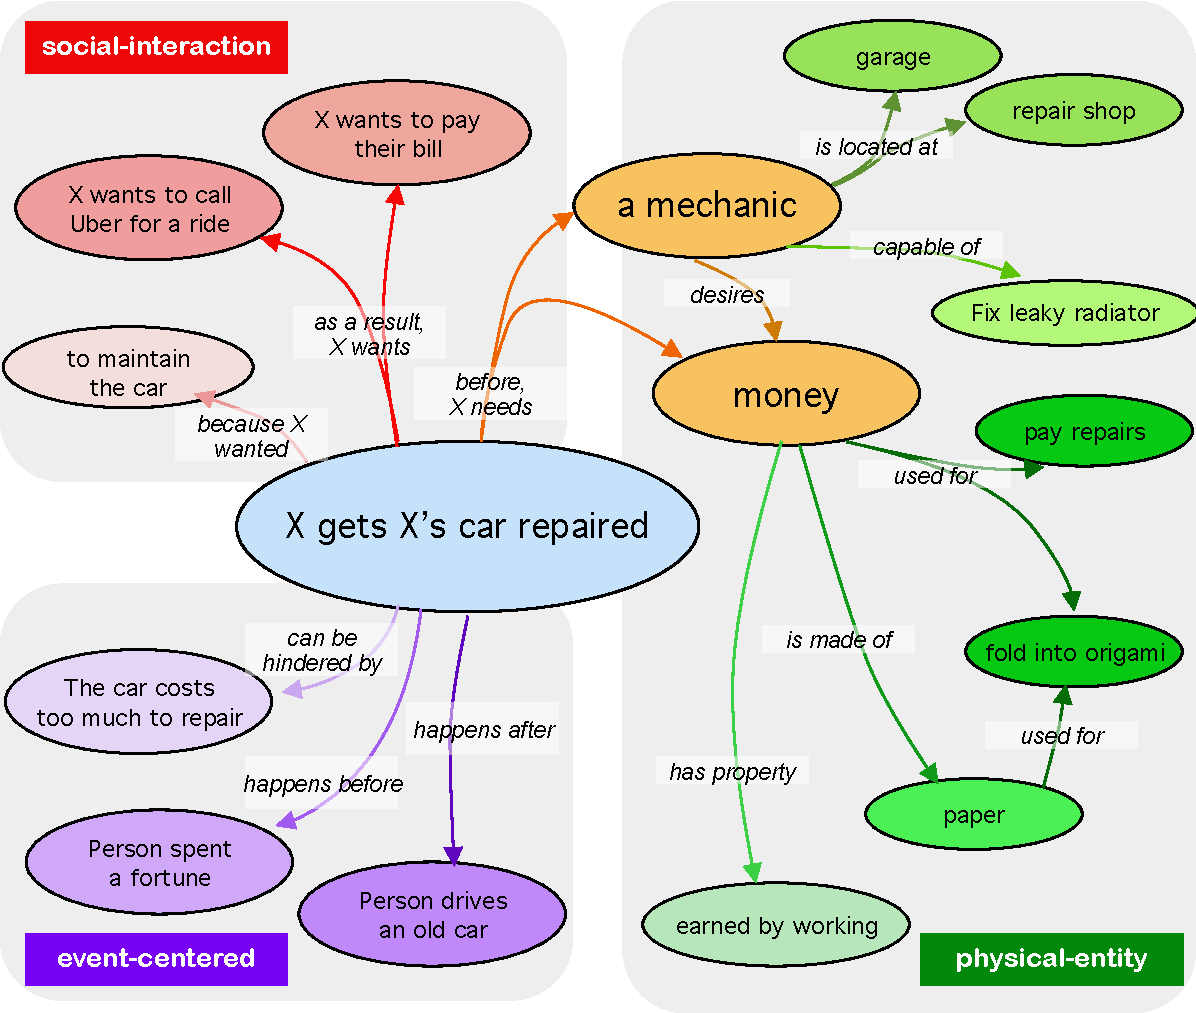
\includegraphics[width=3in]{figures/atomic2020_fig1.pdf}
            \caption{A tiny subset of \atomicTT{}, a large atlas of social and physical commonsense relations. Relations in the top-left quadrant reflects relations from \atomic{}.}
            \label{fig:large_example}
        \end{figure}
    \end{frame}
    
    \begin{frame}
        \frametitle{\textbf{\atomicTT{} Relation}}
        \begin{table}[t]
            \resizebox{0.35\textwidth}{!}{
            \small
            \centering
            \setlength\tabcolsep{3pt}
            \begin{tabular}{p{1em}p{4.5em}p{5.5em}p{9.5em}r}
            \toprule
            &\textbf{Head}  & \textbf{Relation} & \textbf{Tail} & \textbf{Size}\\
            \midrule
            % \multirow{7}{*}{\rotatebox[origin=c]{90}{ Entity-Related}}
            %\multicolumn{4}{l}{\textsc{Physical-Entity Commonsense}}\\
            %\midrule
            \multirow{10}{*}{\rotatebox[origin=rb]{90}{{\color{darkgreen}\textsc{Physical-Entity}}}} & \multirow{5}{*}{bread} & ObjectUse & make french toast & $165{,}590$\\ % attract ants
            \cmidrule{3-5}
            & & AtLocation$^*$ & basket; pantry & $20{,}221$\\
            \cmidrule{3-5}
            & & MadeUpOf & dough; wheat  & $3{,}345$\\
            \cmidrule{3-5}
            & & HasProperty$^*$ & cooked; nice to eat & $5{,}617$\\
            \cmidrule{2-5}
            &\multirow{4}{*}{baker} & CapableOf$^*$ & coat cake with icing & $7{,}968$\\
            \cmidrule{3-5}
            & & Desires$^*$ & quality ingredients & $2{,}737$\\
            \cmidrule{3-5}
            & & Not Desires$^*$ & bad yeast & $2{,}838$\\
            \midrule
            \midrule
            % \multirow{7}{*}{\rotatebox[origin=c]{90}{Event-Related}}
            %\multicolumn{4}{l}{\textsc{Event-Centered Commonsense}}\\
            %\midrule
            \multirow{10}{*}{\rotatebox[origin=rb]{90}{{\color{violet}\textsc{Event-Centered}}}}  & \multirow{8}{*}{\makecell{X runs out\\of steam}} & IsAfter & X exercises in the gym & $22{,}453$\\
            \cmidrule{3-5}
            & & HasSubEvent & become tired  & $12{,}845$\\
            \cmidrule{3-5}
            & & IsBefore & X hits the showers & $23{,}208$\\
            \cmidrule{3-5}
            & & HinderedBy & drinks too much coffee & $106{,}658$\\
            \cmidrule{3-5}
            & & Causes & takes a break & $376$\\
            \cmidrule{3-5}
            & & xReason & did not eat breakfast & $334$ \\

            \multirow{12}{*}{\rotatebox[origin=rb]{90}{{\color{myred}\textsc{Social-Interaction}}}}  & \multirow{7}{*}{\makecell{X runs out\\of steam}} & xNeed & do something tiring & $128{,}955$ \\
            \cmidrule{3-5}
            & & xAttr & old; lazy; lethargic  & $148{,}194$\\
            \cmidrule{3-5}
            & & xEffect & drinks some water & $115{,}124$\\
            \cmidrule{3-5}
            & & xReact & tired & $81{,}397$\\
            \cmidrule{3-5}
            & & xWant & to get some energy & $135{,}360$ \\
            \cmidrule{2-5}
            & \multirow{5}{*}{\makecell{X votes\\for Y}} & xIntent & to give support & $72{,}677$\\
            \cmidrule{3-5}
            & & oEffect & receives praise & $80{,}166$\\
            \cmidrule{3-5}
            & & oReact & grateful; confident  & $67{,}236$\\
            \cmidrule{3-5}
            & & oWant & thank X; celebrate   & $94{,}548$\\
            \bottomrule
            \end{tabular}}
            \caption{Relations in \atomicTT{} along with illustrative examples and their respective size. Relations that reflect semantically identical categories to \conceptnet{} is marked with an asterisk ($^*$).}
            \label{tab:atomic2020-newrelations}
        \end{table}

    \end{frame}
    
    \begin{frame}
        \frametitle{\textbf{Accuracy Assessment}}
        \begin{table}[t]
                \center
                \small
                \begin{tabular}{lrrr}
                    \toprule
                    \textbf{Knowledge Base} & \textbf{Accept}	& \textbf{Reject}	&\textbf{No Judgment}\\
                    \midrule
                    $\atomicTT$   & \textbf{91.3} & \textbf{6.5} & 2.2\\
                    $\atomic$     & 88.5 & 10.0 & 1.5\\
                    $\conceptnet$ & 88.6 & 7.5 & 3.9\\
                    $\transomcs$  & 41.7 & 53.4 & 4.9\\
                    \bottomrule
                \end{tabular}
            \caption{\textbf{Accuracy} - Percentage ($\%$) of tuples in the knowledge base evaluated by human crowdworkers as either always true or likely (Accept), farfetched/never or invalid (Reject), or unclear (No Judgment).}
            \label{tab:precision-results}
        \end{table}
    \end{frame}
 
     \begin{frame}
        \frametitle{\textbf{Accuracy Assessment (Breakdown)}}
        \begin{table}[t]
            \resizebox{0.4\textwidth}{!}{
            \small
            \setlength\tabcolsep{3pt} 
            \begin{tabular}{ccccc}
                \toprule
                \textbf{\atomicTT{}} & \textbf{\atomic{}} & \textbf{\textit{Relation}} & \textbf{CN} & \textbf{T-OMCS} \\
                \midrule                  
                \textbf{92.3} &  & AtLocation* & 89.4 & \cellcolor{gray!25} 34.3 \\
                \textbf{93.9} &  & CapableOf* & \cellcolor{gray!25} 84.4 & \cellcolor{gray!25} 50.0 \\
                \textbf{94.6} &  & Causes & \cellcolor{gray!25} 90.0 & \cellcolor{gray!25} 50.0 \\
                \textbf{96.9} &  & Desires* & 96.3 & \cellcolor{gray!25} 48.2 \\
                \textbf{93.9} &  & HasProperty* & \cellcolor{gray!25} 86.3 & \cellcolor{gray!25} 52.4 \\
                82.3 &  & ObjUse/UsedFor & \cellcolor{gray!55} \textbf{96.3} & \cellcolor{gray!25} 31.6 \\
                \textbf{98.5} &  & NotDesires* & 96.3 &  \\
                \textbf{96.9} &  & HasSubevent & \cellcolor{gray!25} 88.1 &  \cellcolor{gray!25} 57.7 \\
                 &  & HasFirstSubevent & \textbf{93.8} & 52.4 \\
                 &  & HasLastSubevent & \textbf{95.6} & 38.2 \\
                 &  & HasPrerequisite & \textbf{94.4} & 30.0 \\
                75.4 &  & MadeUpOf/MadeOf & \cellcolor{gray!55} \textbf{88.1} & \cellcolor{gray!25} 15.9  \\
                 &  & PartOf & \textbf{71.9} & 46.5 \\
                 &  & HasA & \textbf{77.5} & 43.5 \\
                \textbf{96.9} &  & HinderedBy &  &  \\
                \textbf{96.2} &  & isAfter &  &  \\
                \textbf{95.4} &  & isBefore &  &  \\
                \textbf{96.2} &  & isFilledBy &  &  \\
                 &  & ReceiveAction & \textbf{84.4} & 56.4 \\
                \textbf{91.5} & 86.3 & oEffect &  &  \\
                \textbf{91.5} & 87.7 & oReact &  &  \\
                88.5 & \textbf{89.5} & oWant &  &  \\
                87.7 & \textbf{91.0} & xAttr &  &  \\
                80.8 & \textbf{87.2} & xEffect &  &  \\
                \textbf{93.1} & 89.9 & xIntent/MotivByGoal & 84.4 & \cellcolor{gray!25} 27.1 \\
                \textbf{87.7} & 85.1 & xNeed &  &  \\
                90.8 & \textbf{91.3} & xReact &  &  \\
                \textbf{96.2} &  & xReason &  &  \\
                82.3 & 88.4 & xWant/CausesDesire & \textbf{90.0} & \cellcolor{gray!25} 35.9 \\
                
                \bottomrule
             \end{tabular}}
            \caption{KG accuracy values broken down by relation. Gray cells indicate statistically significant difference from \atomicTT{} values. Dark gray cells signal instances where \atomicTT{} values are significantly higher than its counterpart KB. Relational \textit{cognates} have been grouped together and \textit{exact matches} are asterisked (*) (cf. Table~\ref{tab:atomic2020-newrelations}).}
            \label{tab:precision:breakdown}
        \end{table}
    \end{frame}

    \begin{frame}
        \frametitle{\textbf{Coverage Assessment}}
        \begin{table}[t]
            \resizebox{0.6\textwidth}{!}{
            \small
            \begin{tabular}{lrrrr}
                \toprule
                 & \multicolumn{4}{l}{\textbf{Target KB$\rightarrow{}$}}\\
                 \cmidrule{2-5}
                \textbf{Source KB$\downarrow{}$}   & \atomic{} & CN& T-OMCS & \atomicTT{} \\
                \midrule                  
                $\atomic$      & -        & 0.1      & 0.0  & 100.0  \\
                $\conceptnet$  & 0.3   & -           & 5.5  & 45.6   \\
                $\transomcs$   & 0.0   & 0.4      & -       & 0.3  \\
                $\atomicTT$    & 60.2   & 9.3      & 1.4  & -        \\
                \bottomrule
            \end{tabular}}
            \caption{\textbf{Coverage Precision} - Average number of times (in $\%$) a tuple in Source KB is found in Target KB.}
            \label{tab:coverage:precision}
        \end{table}
        
        \begin{table}[t]
            \resizebox{0.6\textwidth}{!}{
            \small
            \begin{tabular}{lrrrr}
                \toprule
                 & \multicolumn{4}{l}{\textbf{Target KB$\rightarrow{}$}}\\
                 \cmidrule{2-5}
                \textbf{Source KB$\downarrow{}$}   & $\atomic$ & CN& T-OMCS & \atomicTT \\
                \midrule                  
                $\atomic$      & - & 0.3      & 0.0  & 60.1  \\
                $\conceptnet$  & 0.1   & -           & 0.3  & 8.9   \\
                $\transomcs$   & 0.0   & 7.6      & -     & 1.3  \\
                $\atomicTT$    & 100.1$^\dagger$   & 47.8      & 0.4  &   - \\
                \bottomrule
            \end{tabular}}
            \caption{\textbf{Coverage Recall} - Average number of times (in $\%$) a tuple in Target KB is found in Source KB. $^\dagger$This value is greater than 100 because multiple tuples in \atomicTT{} can map to the same tuple in \atomic. }
            \label{tab:coverage:recall}
        \end{table}
    \end{frame}
    
    \begin{frame}
        \frametitle{\textbf{Human Evaluation} (Crowdsource, \$15 per hour)}
        \begin{table}[t]
            \resizebox{0.7\textwidth}{!}{
            \setlength\tabcolsep{3pt} 
            \begin{tabular}{llrrr}
                \toprule
                 \textbf{KG}           &   \textbf{Model}             & \textbf{Accept} & \textbf{Reject} & \textbf{\makecell{No\\Judgm.}} \\
                \midrule            
                
                 \multirow{4}{*}{\atomicTT{}} 
                 & \gptxl{}        & 36.6                    & 62.5                   & 0.9                           \\
                   & \gpttt{} & 73.0 & 24.6 & 2.5       \\
                 & \cometgptxl{} & 72.5                    & 26.6                   & 0.9                           \\
                            & \cometbart{}    & \textbf{84.5}                    & \textbf{13.8}                   & 1.7                           \\
                \midrule
                      & \gptxl{}        & 38.3                    & 61.2                   & 0.4                           \\
                \atomic{}            & \cometgptxl{} & 64.1                    & 34.7                   & 1.2                           \\
                            & \cometbart{}    & \textbf{83.1}                    & \textbf{15.3}                   & 1.6                           \\
                \midrule
                  & \gptxl{}        & 50.3                    & 42.1                   & 7.7                           \\
                \conceptnet{}            & \cometgptxl{} & 74.5                    & 19.0                   & 6.4                           \\
                            & \cometbart{}    & \textbf{75.5}                    & \textbf{17.9}                   & 6.6                           \\
                \midrule
                   & \gptxl{}        & \textbf{28.7}                    & \textbf{53.5}                   & 17.8                           \\
                 \transomcs{}           & \cometgptxl{} & 26.9                    & 60.9                   & 12.2                           \\
                            & \cometbart{}    & 23.8                    & 65.9                   & 10.3                  \\
                            
                \bottomrule
            \end{tabular}}
        \caption{Human evaluation of generation accuracy ($\%$). Each model uses greedy decoding to generate the \emph{tail} of 5K randomly-sampled test prefixes (\emph{head}, \emph{relation}) from each knowledge graph. \gptxl{}, \gpttt{} and BART have 1.5B, 175B and 440M parameters, respectively.}
        \label{tab:human-eval-generations}
        \end{table}        
    \end{frame}
    
    \begin{frame}
        \frametitle{\textbf{Automatic Evaluation}}
        \begin{table}[t]
            \centering
            \resizebox{1.\textwidth}{!}{
            \small
            \begin{tabular}{llcccccccc}
                \toprule
                                &       &   Bleu-1 &   Bleu-2 &   Bleu-3 &   Bleu-4 &   METEOR &   ROUGE-L &   CIDEr &   BERT Score \\
                 \midrule
                 \multirow{2}{*}{\atomicTT{}} & \cometgptxl{} &   0.401 &    0.247 &    0.168 &    0.123 &    0.288 &     0.473 &   0.620 &        0.632 \\
                 & \cometbart{}       &   \bf 0.462 &    \bf 0.280 &    \bf 0.182 &    \bf 0.124 &    \bf 0.325 &    \bf 0.486 &   \bf 0.632 &        \bf 0.636 \\
                  \midrule
                 \multirow{2}{*}{\atomic{}} & \cometgptxl{}     &     0.429 &    0.300 &    0.225 &    \bf 0.187 &    0.297 &     0.527 &   0.754 &        0.638 \\
                 & \cometbart{}            &     \bf 0.521 &    \bf 0.330 &    0.225 &    0.164 &    \bf 0.351 &    \bf  0.552 &  \bf  0.766 &     \bf    0.650 \\
                  \midrule
                 \multirow{2}{*}{\conceptnet{}} & \cometgptxl{} &    0.152 &   \bf  0.115 &  \bf   0.092 &  \bf   0.080 &  \bf   0.131 &   \bf   0.193 &  \bf  0.421 &      \bf   0.552 \\
                 & \cometbart{}        &  \bf   0.169 &    0.108 &    0.069 &    0.046 &    0.127 &     0.180 &   0.350 &        0.532 \\
                  \midrule
                 \multirow{2}{*}{\transomcs{}} & \cometgptxl{} &     0.298 &    0.000 &    0.000 &    0.000 &    0.179 &     0.300 &   0.249 &        0.677 \\
                 & \cometbart{}         &    \bf  0.351 &   \bf  0.216 &   \bf  0.004 &    0.000 &  \bf   0.201 &   \bf   0.352 & \bf   0.298 &      \bf   0.681 \\
                 \bottomrule
            \end{tabular}}
            \caption{Automated metrics for the quality of the \emph{tail} generations for the knowledge models \cometgptxl{} and \cometbart{}. Each approach uses greedy decoding for all test prefixes for each KG. Similar results were obtained on the 5K sampled prefixes that were randomly selected for the human evaluation.}
            \label{tab:auto-eval-full-test}
        \end{table}
    \end{frame}
    
    \begin{frame}
        \frametitle{\textbf{Discussion I}}
        \begin{block}{\textbf{Do pretrained language models already encode commonsense knowledge?}}
            The COMET training paradigm proposed by can perhaps be viewed less as a means of learning \textit{knowledge} from KGs, and more as a method of learning an \textit{interface} for language models to hypothesize encoded knowledge through language generation. We look forward to future work in this space that attempts to disentangle these two ideas.
        \end{block}
    \end{frame}
    
    \begin{frame}
        \frametitle{\textbf{Discussion II}}
        \begin{block}{\textbf{What considerations should be made when designing commonsense knowledge resources?}}
            Because certain types of knowledge are already encoded and expressible by pretrained language models, CSKG designers should focus on collecting examples and categories of knowledge that are less likely to be known by language models. For example, of the 378 test tuples evaluated by the \gptxl{} zero-shot model that contained the \HinderedBy{} relation, only 1.3\% were deemed plausible by human raters -- jumping to 85\% plausibility for \cometbart{} -- pointing to an advantage in constructing \atomicTT{} with this relationship in mind or per-relation accuracy.
        \end{block}
    \end{frame}

\section[HEC]{\textbf{Hashtags, Emotions, and Comments}}
    \begin{frame}
        \frametitle{\textbf{Hashtags, Emotions, and Comments}}
        \begin{figure}
            \centering
            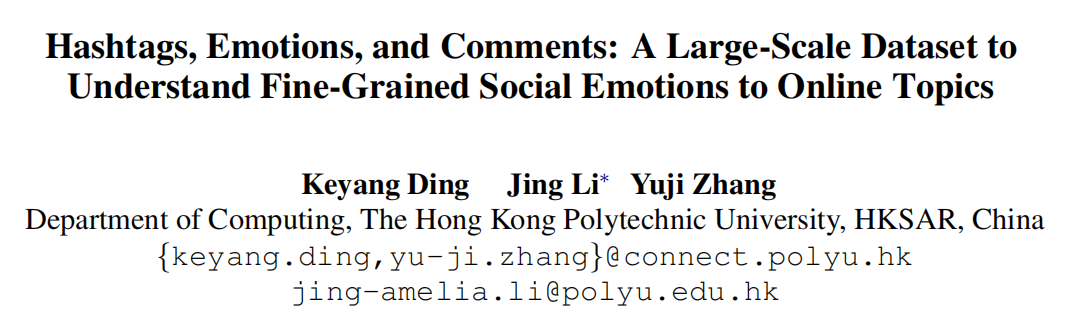
\includegraphics[width=4in]{figures/HEC_info.png}
            \caption{Paper Info \cite{ding_hashtags_2020}}
            \label{fig:HEC_info}
        \end{figure}
        \blfootnote{[8] Keyang Ding, Jing Li and Yuji Zhang. Hashtags, Emotions, and Comments: A Large-Scale Dataset to Understand Fine-Grained Social Emotions to Online Topics. EMNLP2020.}
    \end{frame}
    
    \begin{frame}
        \frametitle{\textbf{Motivations}}
        \begin{itemize}
            \item Most of the related work focus on the feelings from writers and the existing studies concerning reader emotions mostly tackle well-written texts, such as news reports.
            \item Limited work has been done to characterize collective feelings from the public (henceforth \textbf{social emotions}) to an online topic described with fragmented and colloquial social media language.
            \item Where some previous efforts gather viewpoints from limited readers through user replies manual annotations, we focus on social emotions reflecting aggregated feelings from large amount of people.
        \end{itemize}
    \end{frame}
    
    \begin{frame}
        \frametitle{\textbf{Task Definition}}
        \begin{figure}
            \centering
            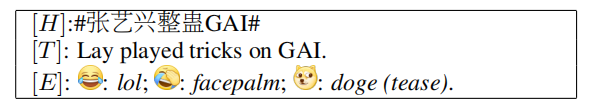
\includegraphics[width=4in]{figures/HEC_task.png}
            \caption{A Weibo hashtag and its resulting social emotions.}
            \label{fig:HEC_task}
        \end{figure}
    \end{frame}
    
    \begin{frame}
        \frametitle{\textbf{Data Collection}}
            Our dataset is built based on a Weibo emotion vote, where it provides users to vote for an emoji from a total of 24 emojis in the form of a questionnaire to represent their feelings to a trending hashtag.
    \end{frame}

    \begin{frame}
        \frametitle{\textbf{Data Collection}}
        First,we tracked the trending hashtags following the everyday Weibo topic summary list from Apr to May 2020.
        \begin{figure}
            \centering
            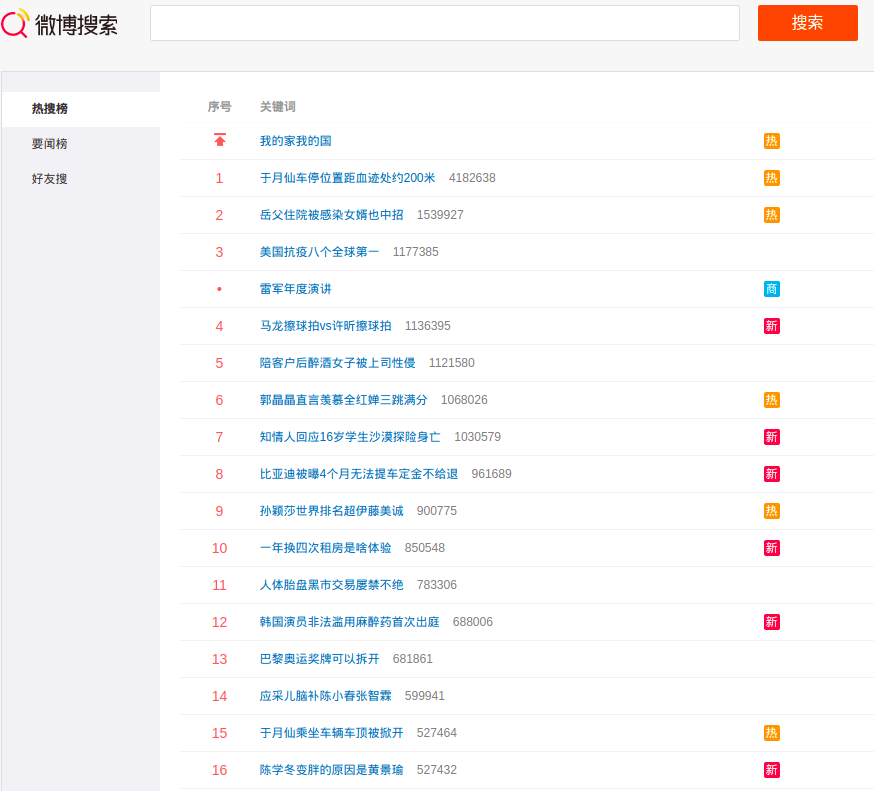
\includegraphics[width=2.4in]{figures/summary.png}
            \caption{Illustration of the summary list.}
            \label{fig:summary}
        \end{figure}
    \end{frame}

    \begin{frame}
        \frametitle{\textbf{Data Collection}}
        Then, we searched and parsed their emotion vote webpage via querying the hashtag in HTTP requests with the selenium package.
        \begin{figure}
            \centering
            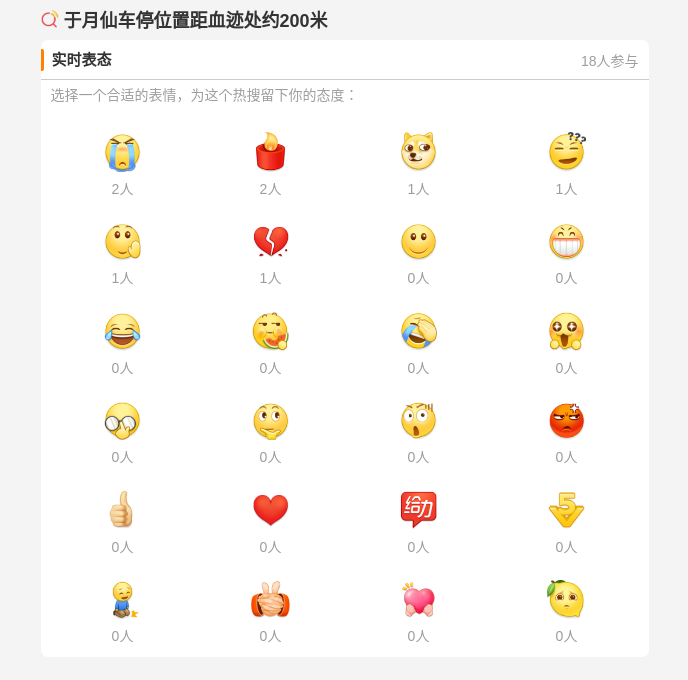
\includegraphics[width=2in]{figures/vote.png}
            \caption{Illustration of the vote webpage.}
            \label{fig:vote}
        \end{figure}
    \end{frame}
    
    \begin{frame}
        \frametitle{\textbf{Data Collection}}
        \begin{itemize}
            \item Next, the crawled pages were parsed and analyzed using lxml package to gather the topics’ emotion voting results. At last, hashtags with less than 100 voters were removed to filter out biased results.
            \item As Weibo only keeps emotions gaining the top three votes, we will hence focus on the top three emotions in the following discussions. These emotions were selected by over 83\% voters on average and can still reflect feelings from the majority.
            \item Furthermore, to access the contexts of hashtags, we collected some user comments involved in a hashtag’s discussion.
        \end{itemize}
    \end{frame}
    
    \begin{frame}
        \frametitle{\textbf{Data Statistics}}
        \begin{figure}
            \centering
            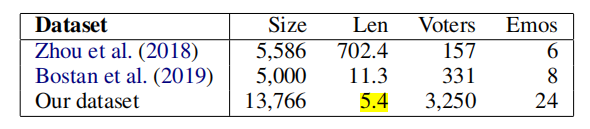
\includegraphics[width=4in]{figures/stat.png}
            \caption{Statistics: our data vs. prior resource. Size and emos are the number of instances and emotion types. Len and voters are the average number of words (after Chinese word segmentation) and the involved voters per instance.}
            \label{fig:stat}
        \end{figure}
    \end{frame}

    \begin{frame}
        \frametitle{\textbf{Data Statistics}}
        \begin{figure}
            \centering
            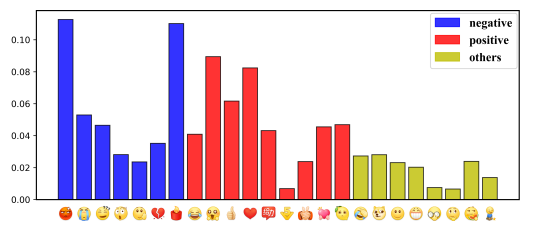
\includegraphics[width=4in]{figures/stat2.png}
            \caption{User preferences over varying emotions.}
            \label{fig:stat2}
        \end{figure}
    \end{frame}
    
    \begin{frame}
        \frametitle{\textbf{Result Analyses}}
        \begin{figure}
            \centering
            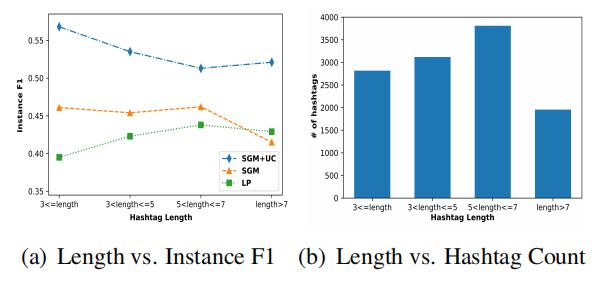
\includegraphics[width=4in]{figures/results.png}
            \caption{Instance F1 (left y-axis) in prediction and training hashtag number (right y-axis) over hashtag length (Chinese word count shown in x-axis).}
            \label{fig:results}
        \end{figure}
    \end{frame}
    
\section*{}
    \begin{frame}
        \begin{center}
            \begin{minipage}{1\textwidth}
                \setbeamercolor{mybox}{fg=white, bg=black!60!green}
                \begin{beamercolorbox}[wd=0.70\textwidth, rounded=true, shadow=true]{mybox}
                    \LARGE \centering Thanks for Listening.
                \end{beamercolorbox}
            \end{minipage}
        \end{center}
        
        \begin{figure}[!t]
            \centering
            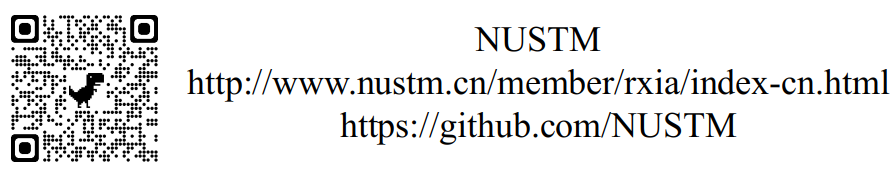
\includegraphics[width=.8\textwidth]{source/nustm_contact.png}
            \label{figure4_ad}
        \end{figure}
    \end{frame}
            
\begin{frame}[allowframebreaks]
    \frametitle{\textbf{References}}
    \bibliographystyle{ieeetr}
    \bibliography{my_bib.bib}
    % \printbibliography[heading=none]
\end{frame}


\end{document}
